\svnid{$Id$}
\chapter{Oxygen Reduction in \Nm{}}
\label{chap:oxygenreduction}
\section{Aerobic Reduction of Oxygen}
\subsection{Introduction}
The first dataset used in the iterative approach to parameter estimation was of a simple oxygen reduction experiment carried out in aerobic conditions. This dataset is the simplest biologically as under aerobic conditions and without the presence of any microaerobic substrates (nitrite or nitric oxide) the only respiratory pathway that is active is the oxygen reducing one. Additionally, the other parts of a respiratory chain influence the oxygen reducing pathway either by competing for electrons, or chemically inhibiting it. The relevant portions of the ETC are shown graphically in Figure \ref{fig:o2_resp_chain}.

\begin{figure}[tbp]
	\centering
	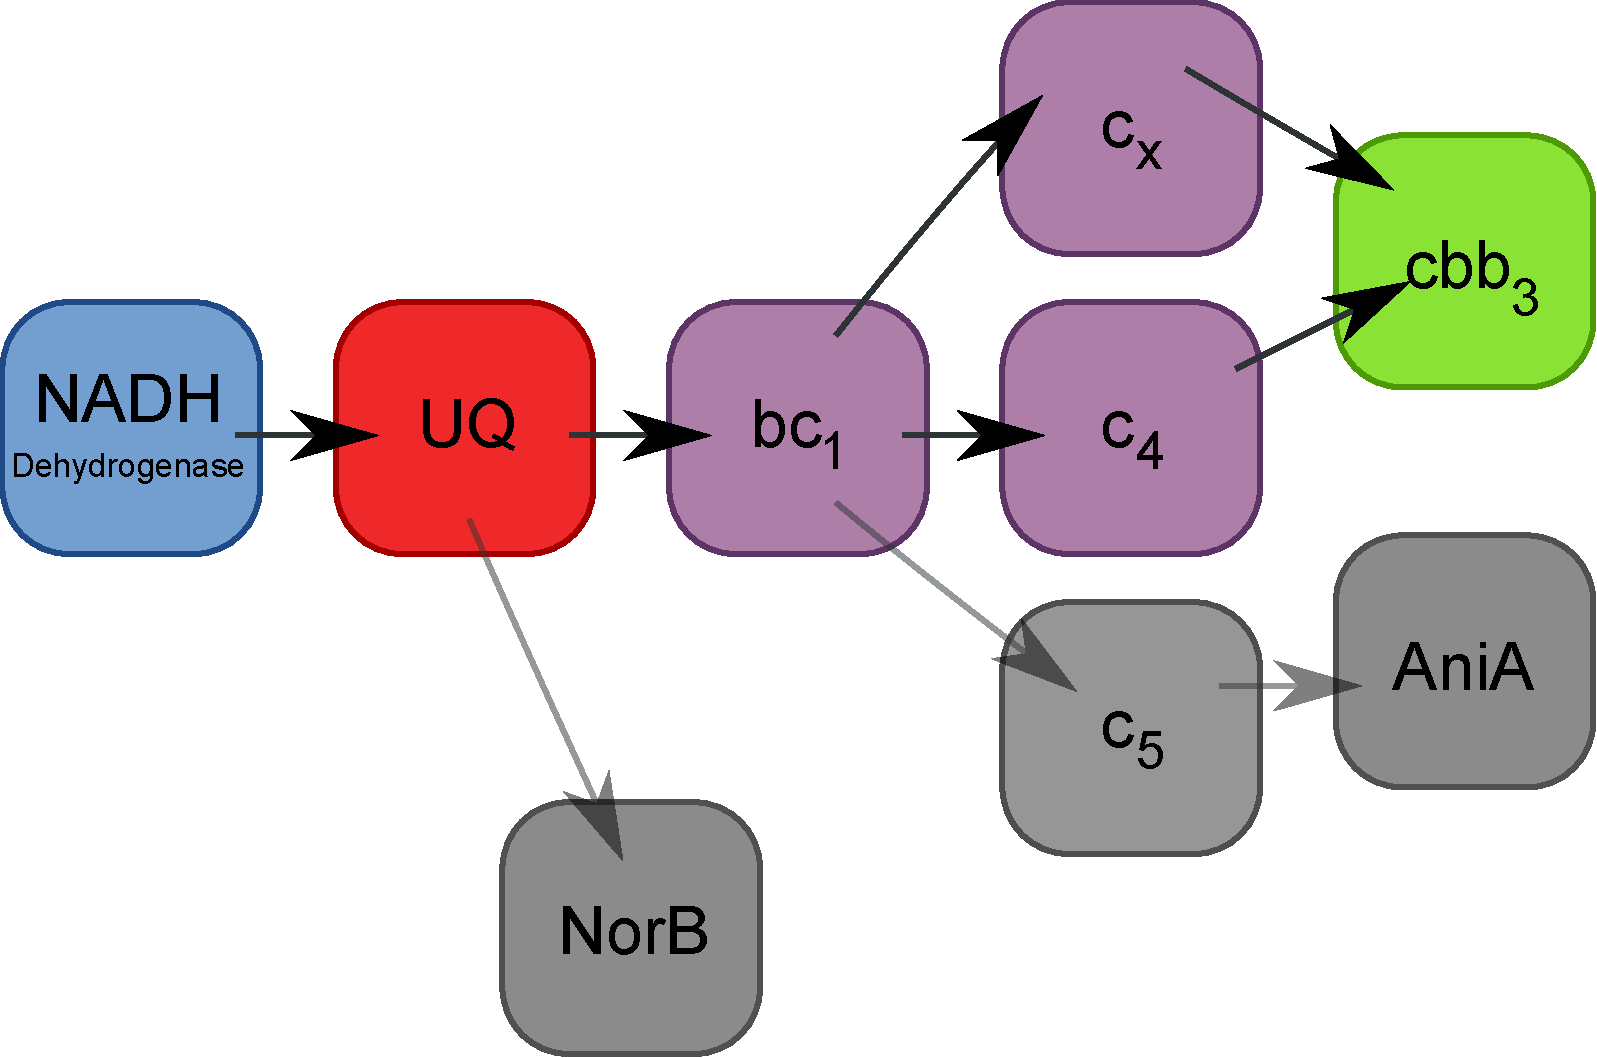
\includegraphics[width=14cm]{05-oxygenreduction/data/o2_resp_chain.pdf}
	\caption[Oxygen reducing electron transport chain of \Nm{}]{{\bf Oxygen reducing electron transport chain of \Nm{}.} This shows the complete electron transport chain of \Nsm{} with the components irrelevant to oxygen reduction greyed out. In the mathematical model all of the purple elements (cytochromes) are amalgamated into one entity.
	\label{fig:o2_resp_chain}}
\end{figure}

The equations that describe this portion of the ETC are:
\begin{eqnarray*}
\frac{d[O_2]}{dt} & = & \beta(1-[O_2]/K_O) - k_{1}[C_a][O_2]\\
\frac{d[Q_a]}{dt} & = & g([Q] - [Q_a]) - l_3[Q_a]([B] - [B_a]) - f[Q_a]([X]-[X_a])\\
\frac{d[X_a]}{dt} & = & -k_3([C] - [C_a] - [C_X])[X_a]  - m_3([A] - [A_a])[X_a] + f[Q_a]([X]-[X_a])\\
\frac{d[C_a]}{dt} & = & k_3([C] - [C_a] - [C_X])[X_a] - k_{1}[C_a][O_2] - k_5[C_a][NO] + k_6[C_X]
\end{eqnarray*}
These equations describe the change in concentration of oxygen over time, which is the experimentally observable value, the reduction state of the quinone pool and the reduction state of the cytochrome ``pool''. This portion of the model involved 13 parameters and variables which were to be estimated (the model actually contains 17 such parameters and variables, but under these conditions the remaining 4 are set to 0 as they are related to nitrite reduction effects). This large number of parameters will clearly result in over-fitting, however this was necessary to generate loose bounds for all of the parameters.

\subsection{Experimental Results}
Generation of oxygen reduction datasets required the growth of MC58 (wild-type \Nsm{}) in aerobic conditions until mid log-phase growth had been achieved. This corresponds to an $\mathrm{OD}_{600}$ of 0.3-0.9 and usually required an incubation period of roughly 3 hours. Once the required cell density had been obtained, the  culture was transferred to the oxygen electrode chamber and recorded the oxygen concentration as the culture respired. At this point the cells are only using whatever amount of oxygen is presently dissolved in the culture medium in addition to that diffusing in through the cap (negligible). Once the culture had used up all its dissolved oxygen, the electrode chamber cap was removed and the culture media aerated using a Pasteur pipette. This restores oxygen levels throughout the culture and allows the bacteria to continue respiring in aerobic conditions. A typical oxygen reduction plot is shown in Figure \ref{fig:oxy_repeatable_chl}. This is split into individual reduction sections, which can then be used as input data for parameter estimation. In many cases if the culture is allowed to become completely anaerobic for a prolonged period of time, the bacteria will die, evidenced by a subsequent lack of oxygen reduction, however this is not always the case as shown in Figure \ref{fig:repeat_oxy_with_delay}.

The experiments used to generate data for oxygen reduction are highly repeatable and consistently generate the same basic result of a linear reduction of oxygen with time.
\begin{figure}[t]
 \centering
 %trim = l b r t
 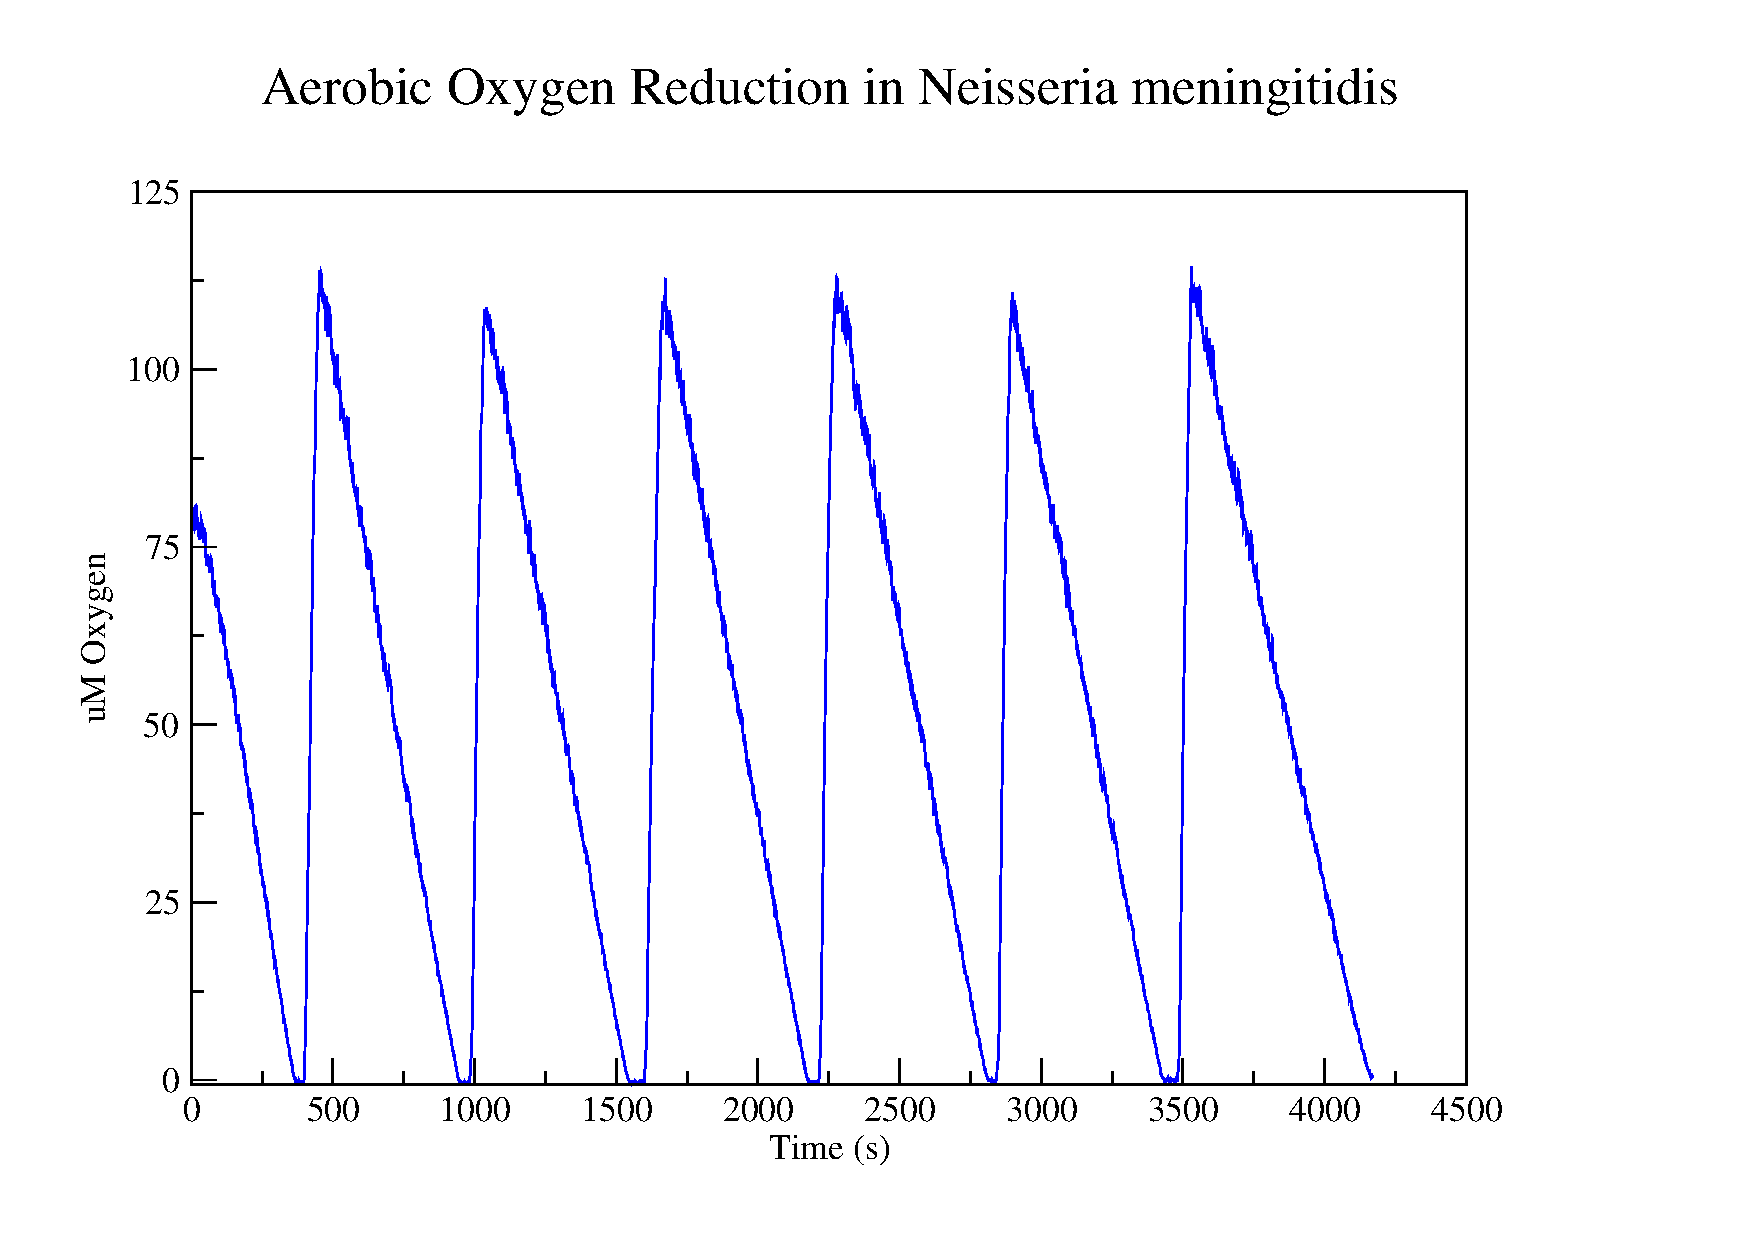
\includegraphics[width=13cm, trim=75px 50px 125px 25px]{./05-oxygenreduction/data/repeatable_o2.pdf}
 % mc58-chl-o2-util.pdf: 842x595 pixel, 72dpi, 29.70x20.99 cm, bb=0 0 842 595
 \caption[Highly repeatable oxygen reduction]{{\bf Highly repeatable oxygen reduction.} This shows an oxygen reducing culture being repeatedly aerated after oxygen depletion with very similar rates of subsequent oxygen reduction
 \label{fig:oxy_repeatable_chl}}
\end{figure}

\begin{figure}[t]
 \centering
 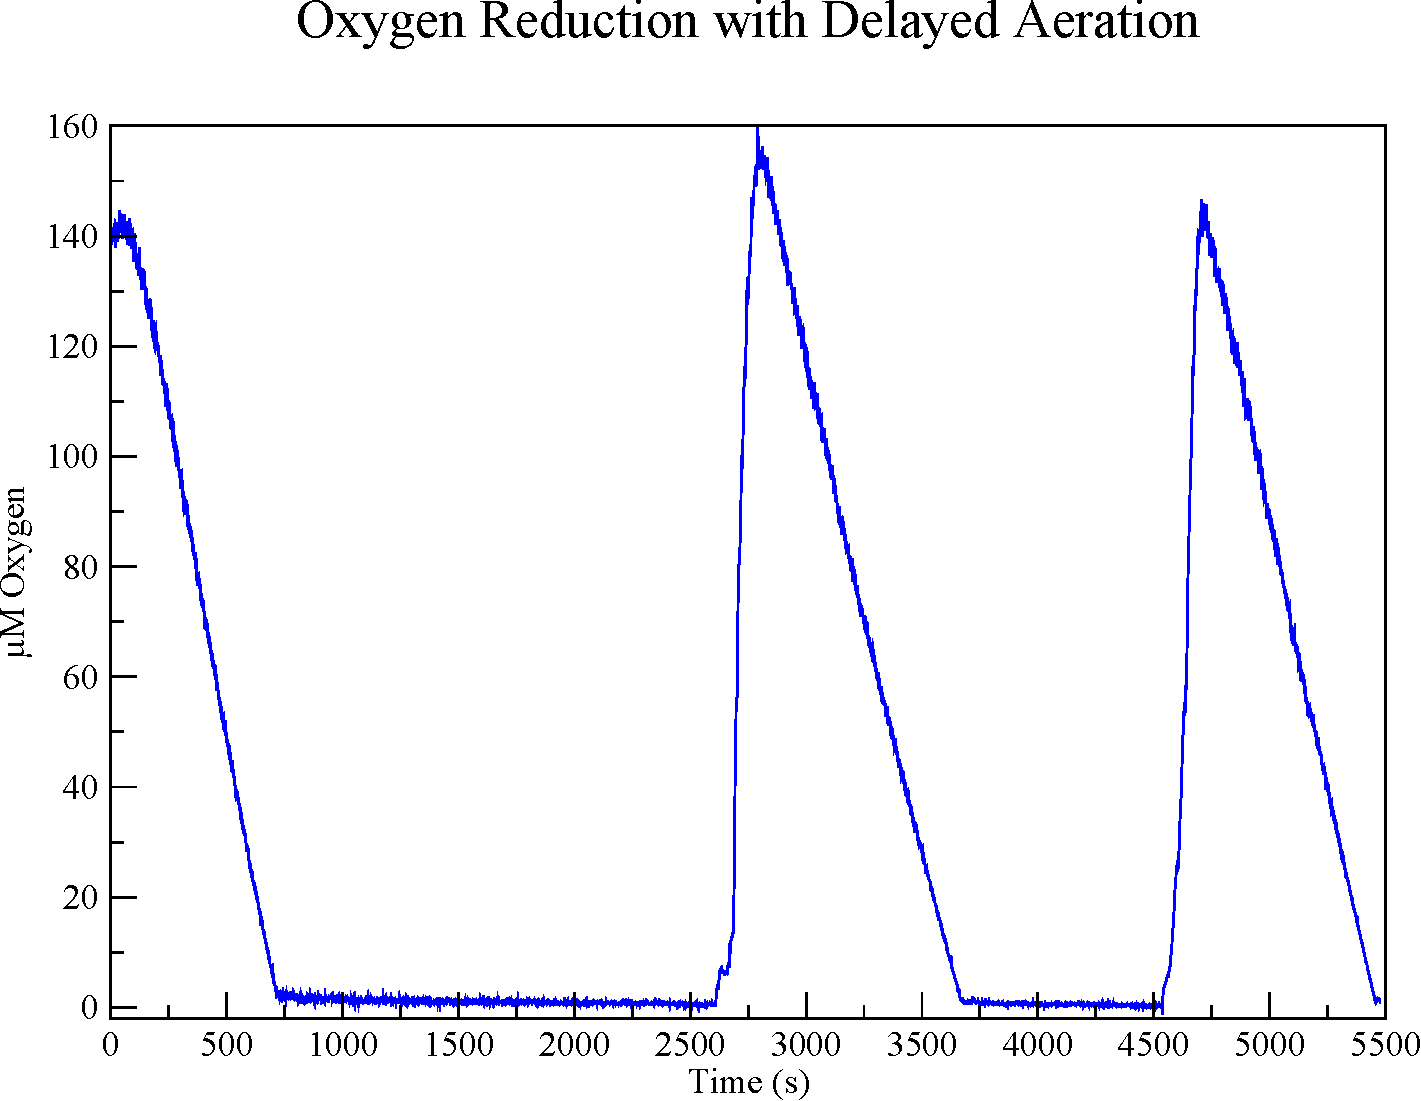
\includegraphics[width=13cm, trim=75px 50px 125px 25px]{./05-oxygenreduction/data/o2_delay.pdf}
 % repeatable-oxygen-utilisation-in-mc58.png: 640x480 pixel, 72dpi, 22.58x16.93 cm, bb=0 0 640 480
 \caption[Aerating oxygen reducing cultures with significant delay]{{\bf Aerating oxygen reducing cultures with significant delay.} The oxygen reducing ability of \Nm{} can be robust as evidenced by the 1000s delays between aeration with no change in subsequent respiration rate. Also of note is that nitric oxide concentration is not changing, suggesting that reduction of nitrite is not occurring either.
 \label{fig:repeat_oxy_with_delay}}
\end{figure}

The oxygen reduction datasets generated and used for parametrising this portion of the mathematical model are shown in Figure \ref{fig:o2data}.

\begin{figure}[p]
 \centering
 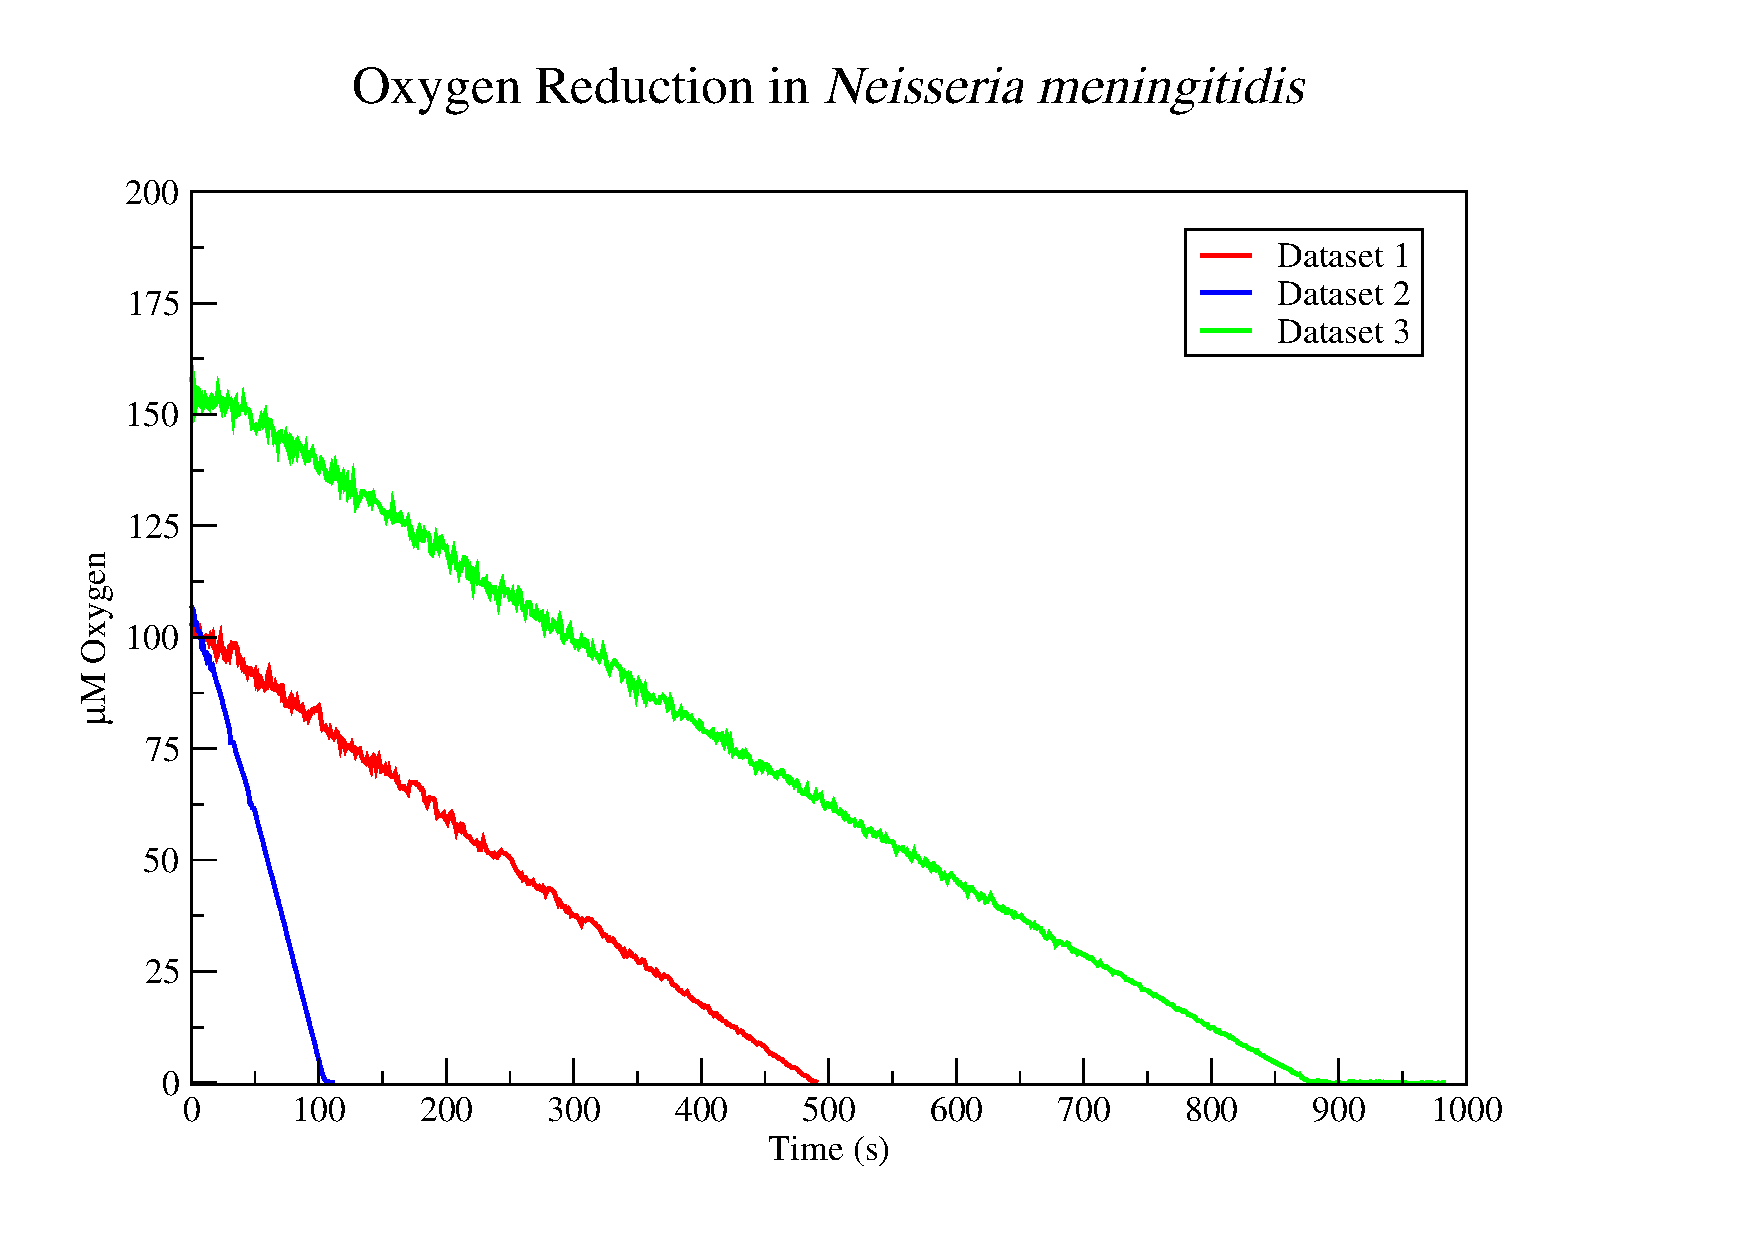
\includegraphics[width=14cm, trim=2cm 1cm 4cm 1cm]{./05-oxygenreduction/data/o2_datasets.pdf}
 % o2sim.eps: 0x0 pixel, 300dpi, 0.00x0.00 cm, bb=0 0 794 595
 \caption[{Oxygen Reduction in \textit{Neisseria meningitidis}.}]{{\bf Oxygen Reduction in \textit{Neisseria meningitidis}.} These three experimental datasets were used as input data for the parameter estimation algorithm. They all show the same linear oxygen reduction. The different rates are due to differing starting cell densities.
 \label{fig:o2data}}
\end{figure}
\afterpage{\clearpage}

\subsubsection{Generation of Prior Probability Distributions}
In accordance with the integrative scheme that was introduced in Chapter \ref{chap:paramest}, An attempt was made to estimate the distributions of the parameters involved in modelling these data. In order to do this probability distributions were needed to act as priors to feed into the estimation system as this is required for a Bayesian approach. These probability distributions were generated from data obtained in the published literature, which is described in Chapter \ref{chap:model}, and preliminary experimental data. It was assumed that all the prior probabilities would be log-normally distributed, therefore the distributions  used were created under the following scheme:
\begin{itemize}
\item Where the literature value had bounds associated with it (i.e. published with $\pm{}$ values), the bounds were assumed to cover $3 \sigma$ of the normal distribution. Thus the variance used for the lognormal distribution is $\left(\frac{bounds}{3}\right)^2$ with narrow upper and lower limits.
\item Where the literature value has no bounds associated with it (i.e. published as a single figure), the bounds were assumed to be $\pm 10\%$ of the literature value, and this was used as $\sigma$. Wider upper and lower limits were used in these cases.
\item Where there are no literature values available, the value was estimated based on preliminary experimental data and bounds of $\pm 10\%$ were used again. In this case upper and lower limits for the distribution were made very wide to try and accommodate for incorrect assumed prior values.
\end{itemize}

\noindent With reference to the above, the values required to create prior probability distributions from Table \ref{tab:ps} in Chapter \ref{chap:model} are shown in Table \ref{tab:oxyProbstat}.

\begin{table}[h]%needs to be 'here' as section is short
\renewcommand{\arraystretch}{1.5}
\begin{center}
\begin{tabular}{cccc|cccc}
\toprule
\textbf{Parameter} && ${\bar{x}}$ & $\sigma$ & \textbf{Parameter} && ${\bar{x}}$ & $\sigma$\\
\midrule
$k_1$ && 415 & 13.83 & X && 3.97 & 0.134\\
$k_3$ && 3 & 0.1 & C && 0.03 & 0.001\\
$\beta$ && 0.00014 & $4.67\times 10^{-06}$ & $Q_a$ && 0.24 & 0.008 \\
g && 0.847 & 0.028 & $X_a$ && 3.176 & 0.105 \\
f && 8.749 & 0.292 & $C_a$ && 0.024 & 0.0008 \\
Q && 0.3 & 0.01\\
\bottomrule
\end{tabular}
\end{center}
\caption[First Prior Probability Table]{{\bf Prior Probability Table} This table shows the prior means and variances used to create lognormal distributions to be used as the prior probability distributions.
\label{tab:oxyProbstat}}
\end{table}

\noindent A graphical representation of the data in Table \ref{tab:oxyProbstat}, the initial probability distributions used to start the Monte-Carlo run are shown in Figure \ref{fig:oxypriors}.% As can be seen, very little information is readily available in the literature to populate the model.

%lbrt
\begin{figure}[p]
 \centering
 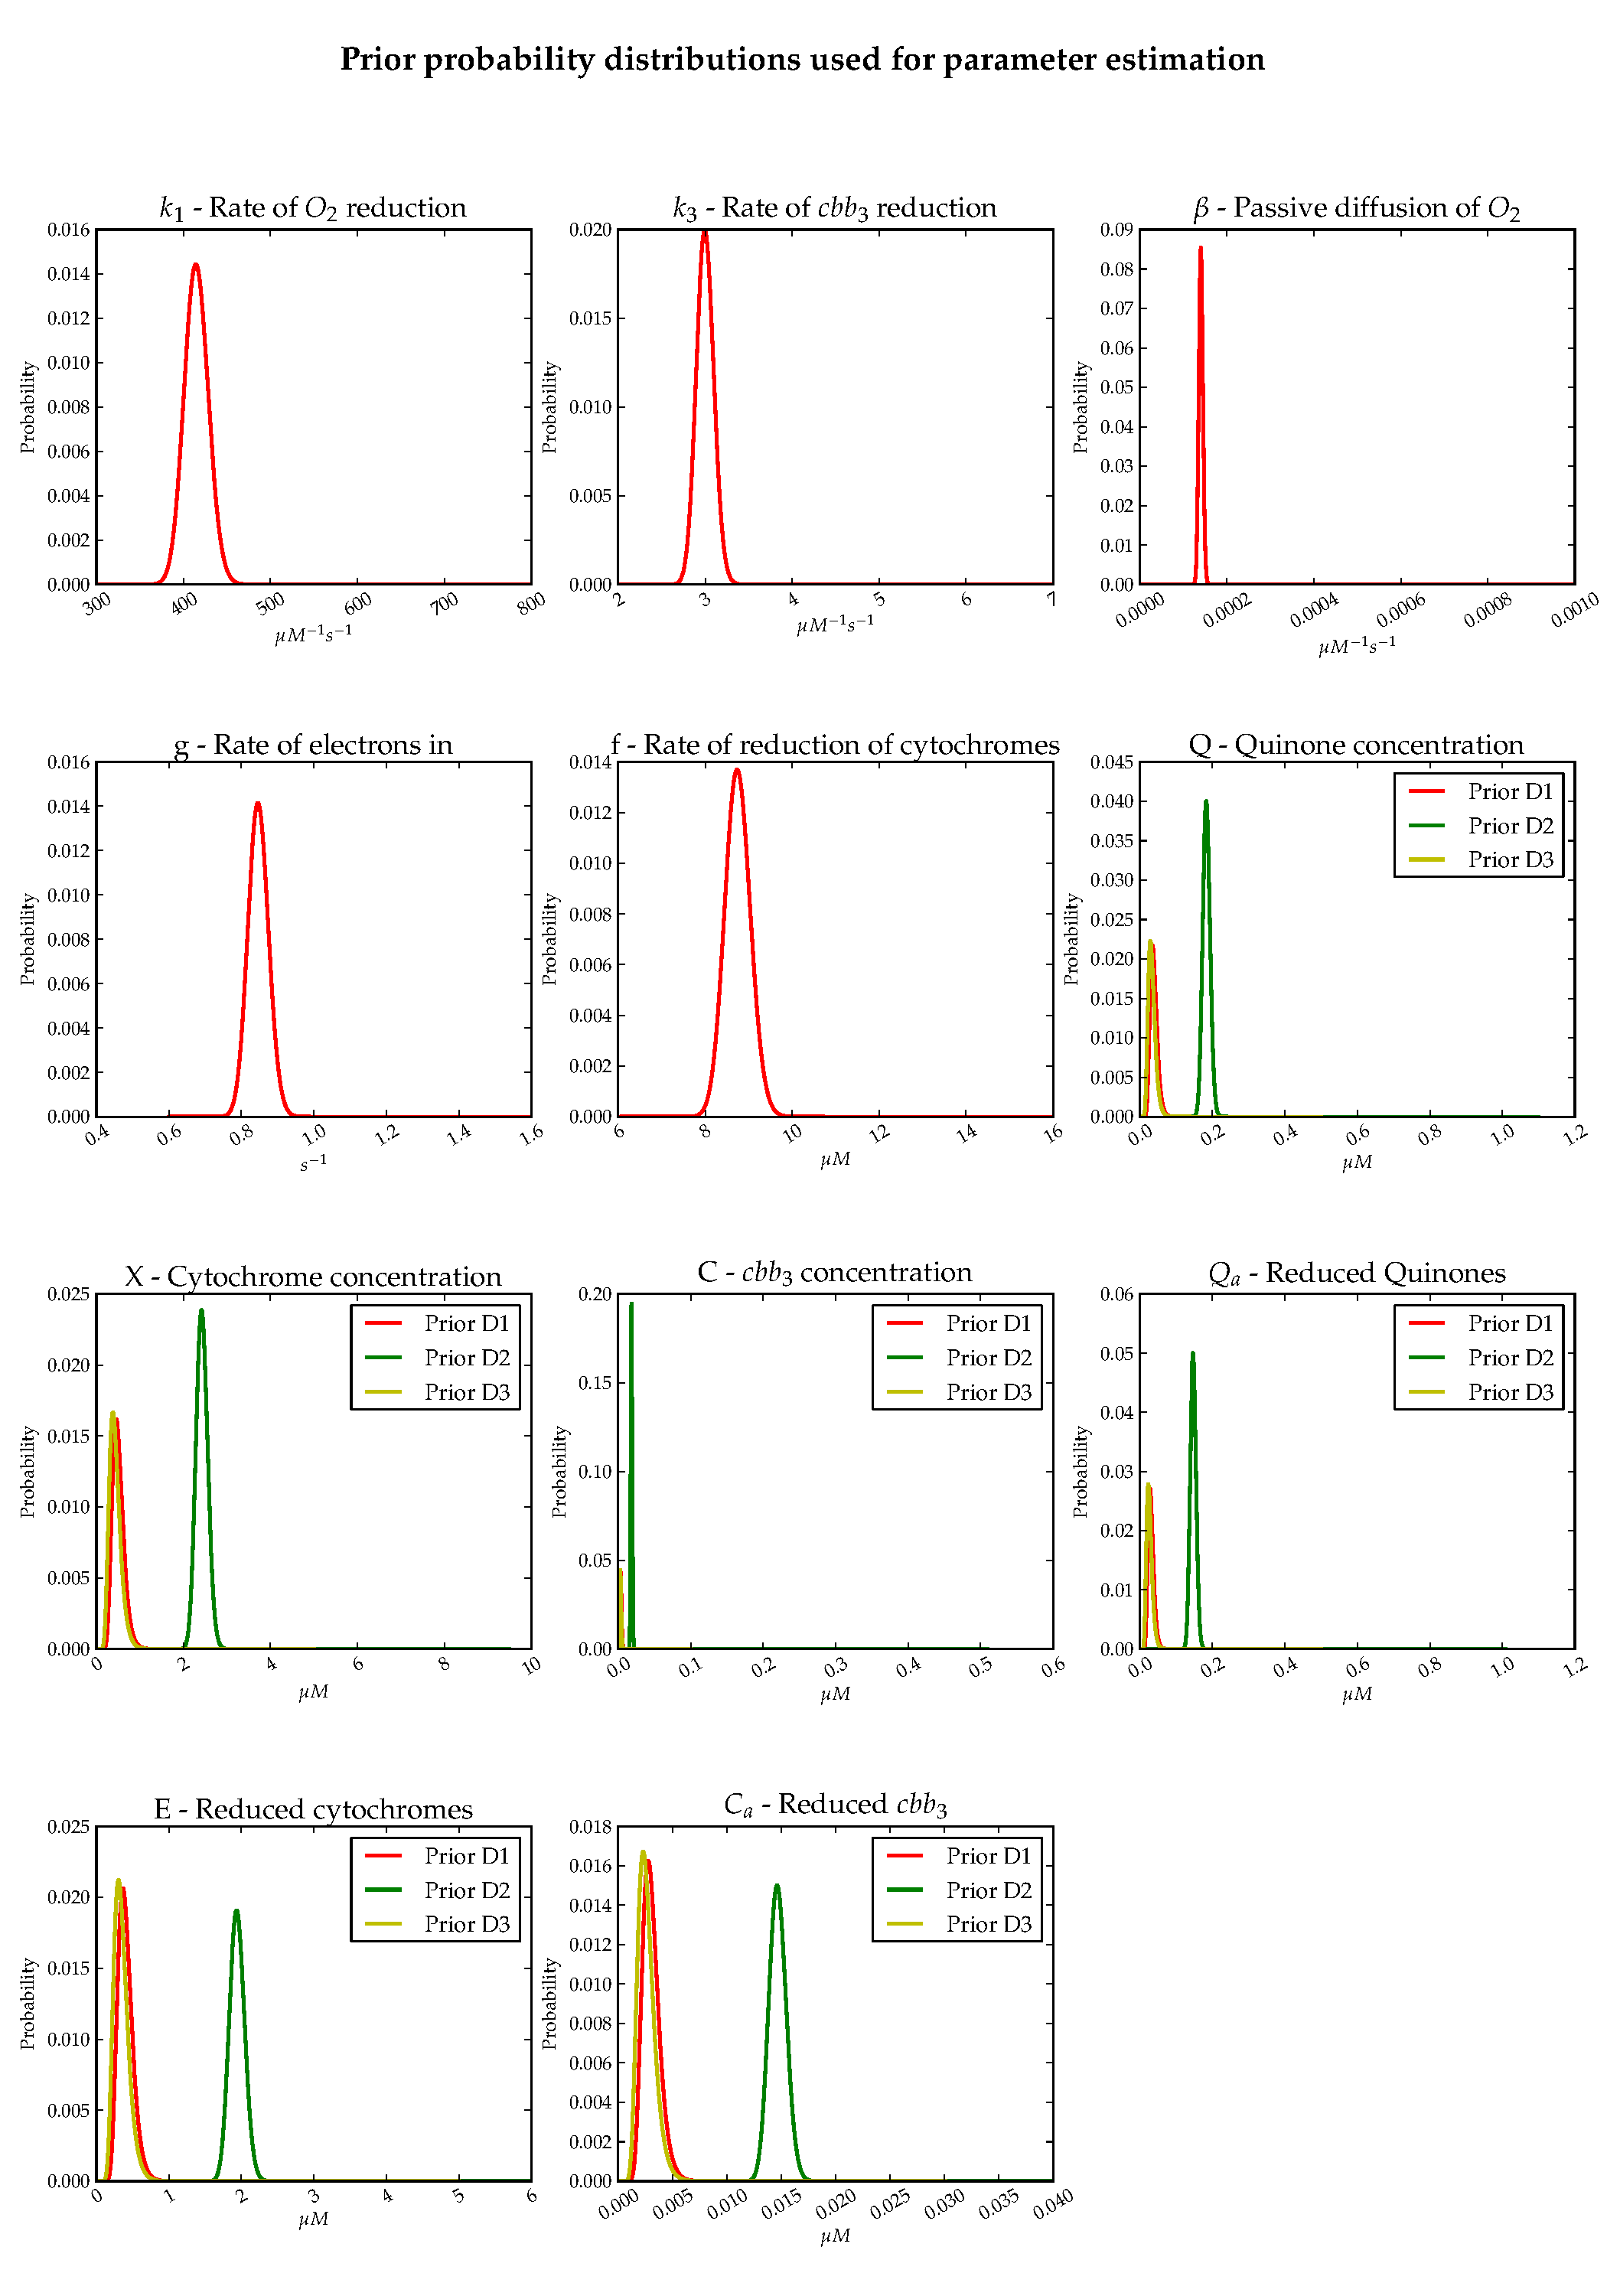
\includegraphics[width=15cm, trim=0cm 0cm 0cm 0cm]{./05-oxygenreduction/data/priors1.pdf}
 % priors.pdf: 1008x1008 pixel, 72dpi, 35.56x35.56 cm, bb=0 0 1008 1008
 \caption[Prior probability distributions for oxygen reduction]{{\bf Prior probability distributions for oxygen reduction}. These are the probability distributions used as priors by the parameter estimation algorithm.
 \label{fig:oxypriors}}
\end{figure}
\afterpage{\clearpage}

\subsubsection{Initial Parameter Estimation Results}
The parameter estimation process produces a large amount of output data which can be processed. Included in these data are the best simulation results from each run. Best is defined here as the simulation with the best goodness-of-fit, i.e. the one with the closest match to the experimental data. For the oxygen reduction training datasets, of which there are 3, each was run 20 times for 20,000 iterations. This lower iteration count was chosen as a compromise between execution time and statistical accuracy. In fact given that the burn-in time for these runs was relatively short, 20,000 iterations still provides plenty of data. A representative example of the simulated data is shown in Figure \ref{fig:o2sim}. This figure was generated from the set of parameters that produced the most fit output compared to the input dataset.

%lbrt
\begin{figure}[p]
 \centering
 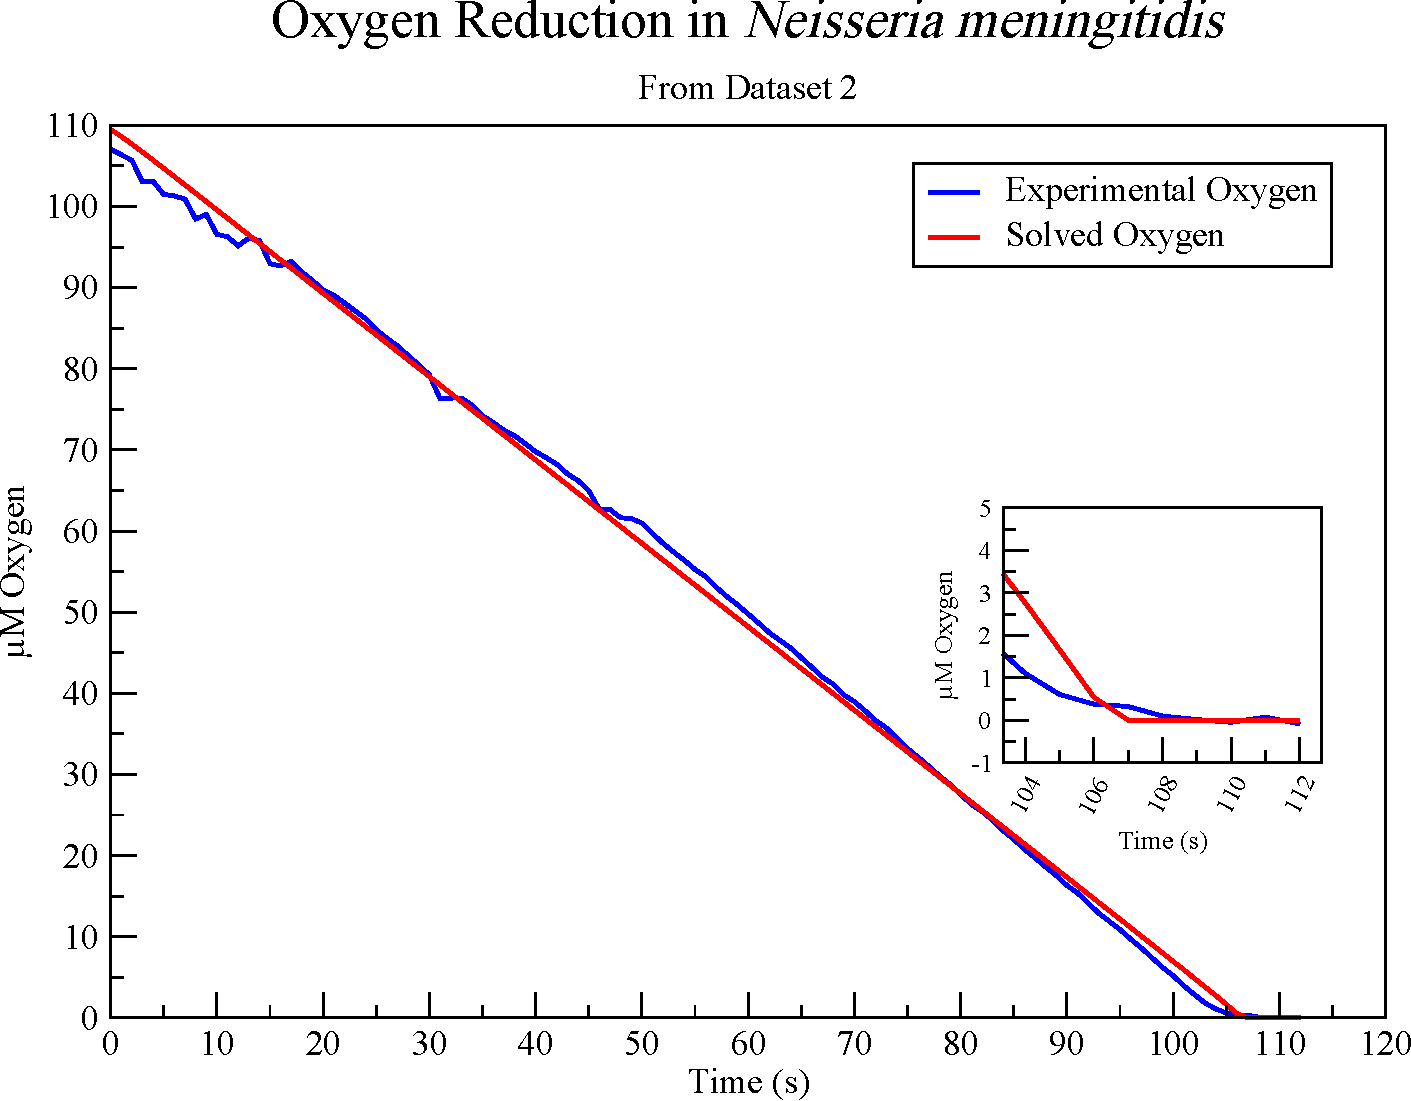
\includegraphics[width=14cm, trim=2cm 1cm 4cm 1cm]{./05-oxygenreduction/data/o2sim.pdf}
 % o2sim.eps: 0x0 pixel, 300dpi, 0.00x0.00 cm, bb=0 0 794 595
 \caption[{Oxygen Reduction in \textit{Neisseria meningitidis}.}]{{\bf Oxygen Reduction in \textit{Neisseria meningitidis}.} This dataset shows the simple linear reduction of Oxygen in aerobic conditions. The high affinity of $\mathrm{cbb}_3$ for oxygen is evidenced by very little non-linearity at low oxygen concentrations. The solved output is a representative result of the parameter estimation system. The inset shows that the solved output is achieving much higher affinity than the experimental data.
 \label{fig:o2sim}}
\end{figure}
\afterpage{\clearpage}
%\begin{figure}[tbp]
 %\centering
 %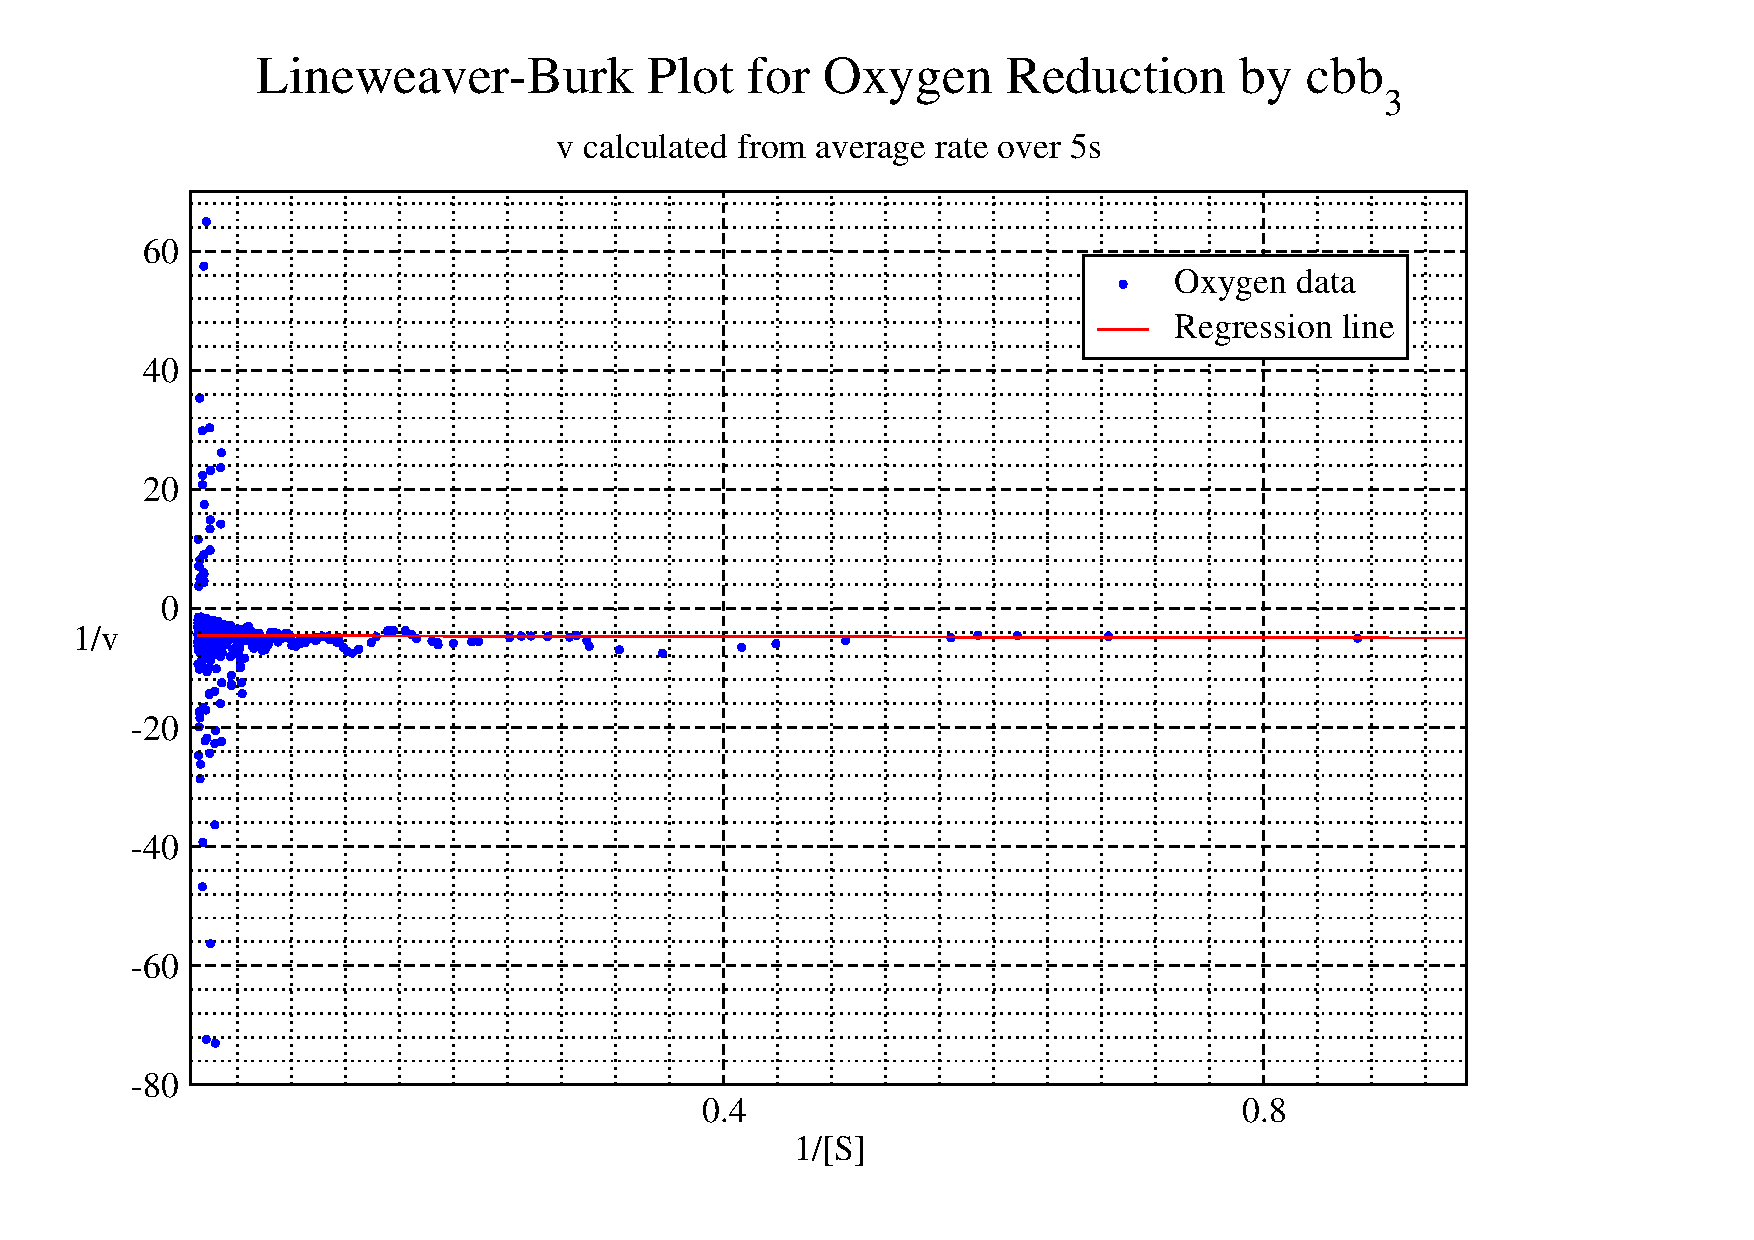
\includegraphics[height=10cm, trim=2cm 1cm 4cm 1cm]{./05-oxygenreduction/data/lbplot.pdf}
 % lbplot.pdf: 842x595 pixel, 72dpi, 29.70x20.99 cm, bb=0 0 842 595
%\end{figure}


Initially the simulation results are not particularly good fits compared to the experimental data and as such have a low goodness-of-fit. The calculation performed actually produces a value that represents the ``badness-of-fit'' related to the distance of the solved data away from the experimental data and accounting for Gaussian noise. As such the quality of the solved data will be given in terms of its ``badness-of-fit'' or \textit{BOF}\nomenclature{BOF}{Badness of Fit}. As the parameter estimation progresses the \textit{BOF} reduces as the simulated result gets closer and closer to the experimental data. Quite often this does not take many iterations and a representative plot showing how the simulation's \textit{BOF} decreases is shown in Figure \ref{fig:oxy_fitness}. The initial period where the \textit{BOF} is high up until the point it settles at a lower value is classed as ``burn-in'' and is discarded when generating posterior distributions.

\begin{figure}[p]
 \centering
 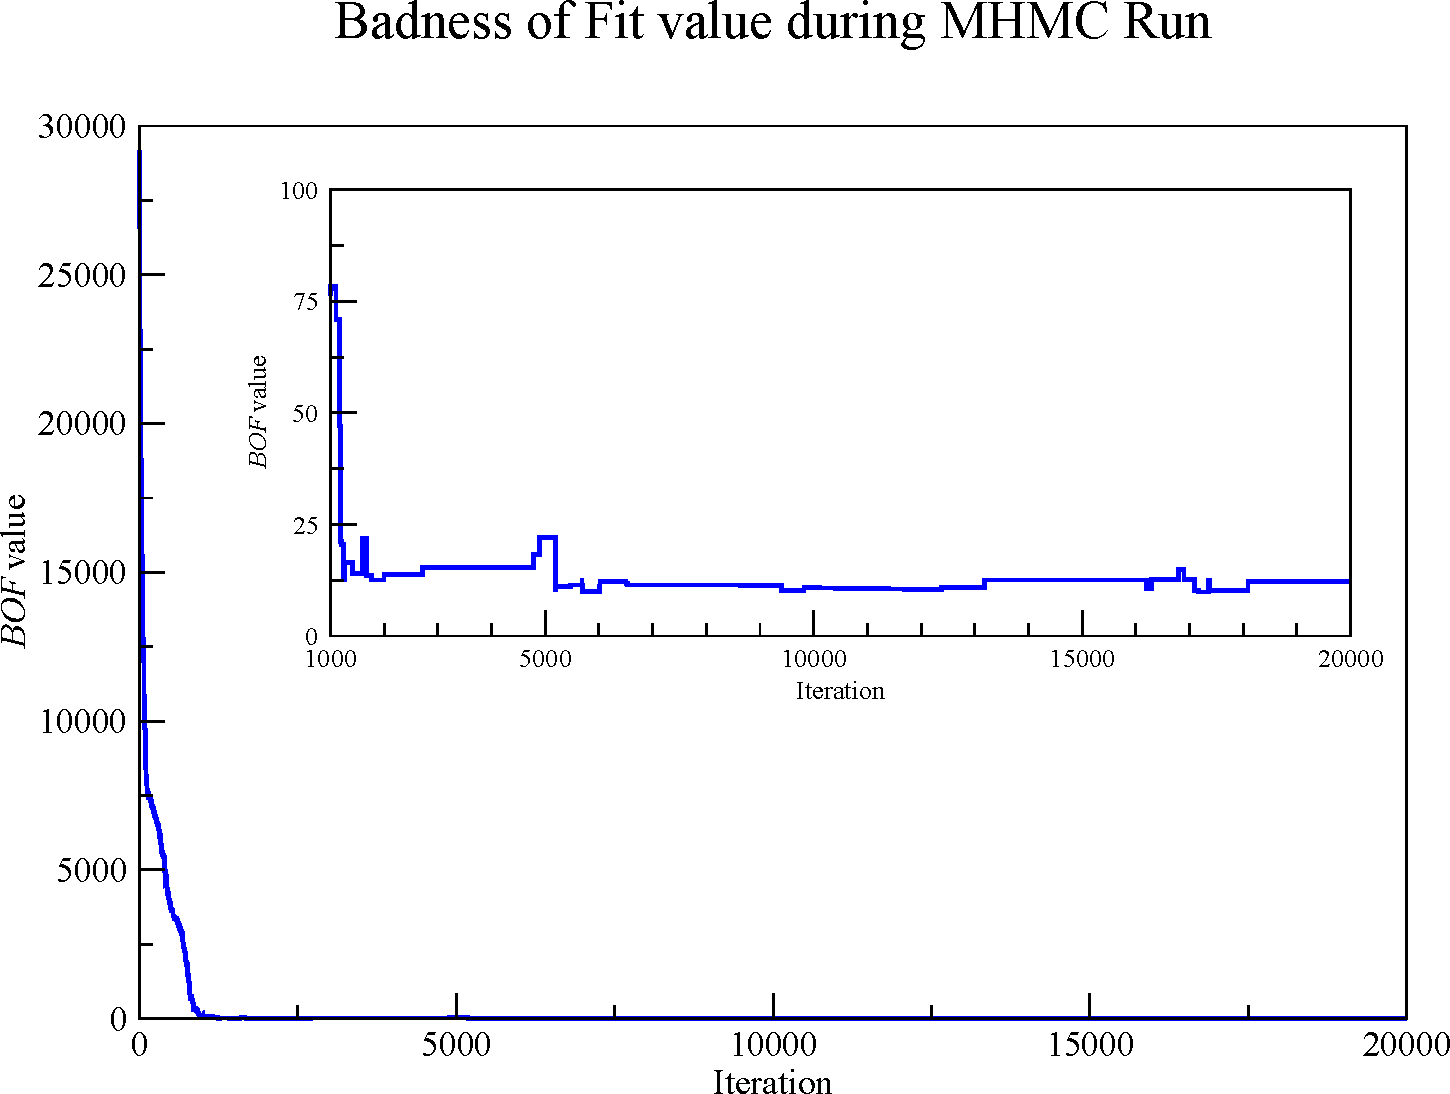
\includegraphics[width=14cm, trim=75px 50px 125px 25px]{./05-oxygenreduction/data/o2_fitness.pdf}
 % repeatable-oxygen-utilisation-in-mc58.png: 640x480 pixel, 72dpi, 22.58x16.93 cm, bb=0 0 640 480
 \caption[Simulation \textit{BOF} improves as parameter estimation progresses]{{\bf Simulation \textit{BOF} improves as parameter estimation progresses.} This is a representative figure constructed from a single run on one dataset. Initially the \textit{BOF} is high showing that the simulated result does not match the experimental dataset. As the parameter estimation algorithm progresses, the \textit{BOF} decreases as the simulated result approaches the experimental dataset. The inset shows a zoomed in view of the \textit{BOF} after the ``burn-in'' process has finished.
 \label{fig:oxy_fitness}}
\end{figure}
\afterpage{\clearpage}

Each of the parameters that are to be estimated produces a trajectory of values for each run of the estimation algorithm. These trajectories are used to generate the posterior probability distributions required for Bayesian inference in subsequent steps. During the ``burn in'' period the parameter values can be observed to change rapidly from one iteration to the next as they approach their optimum values. Once the ``burn in'' has completed the values settle and produce largely flat trajectories with minor deviations around the optimum value. This settled region is used as the source for generating the posterior probability distributions.

Figure \ref{fig:k3s} shows the trajectories from each simulation run on a single dataset for the $k_3$ parameter.

\begin{figure}[p]
 \centering
 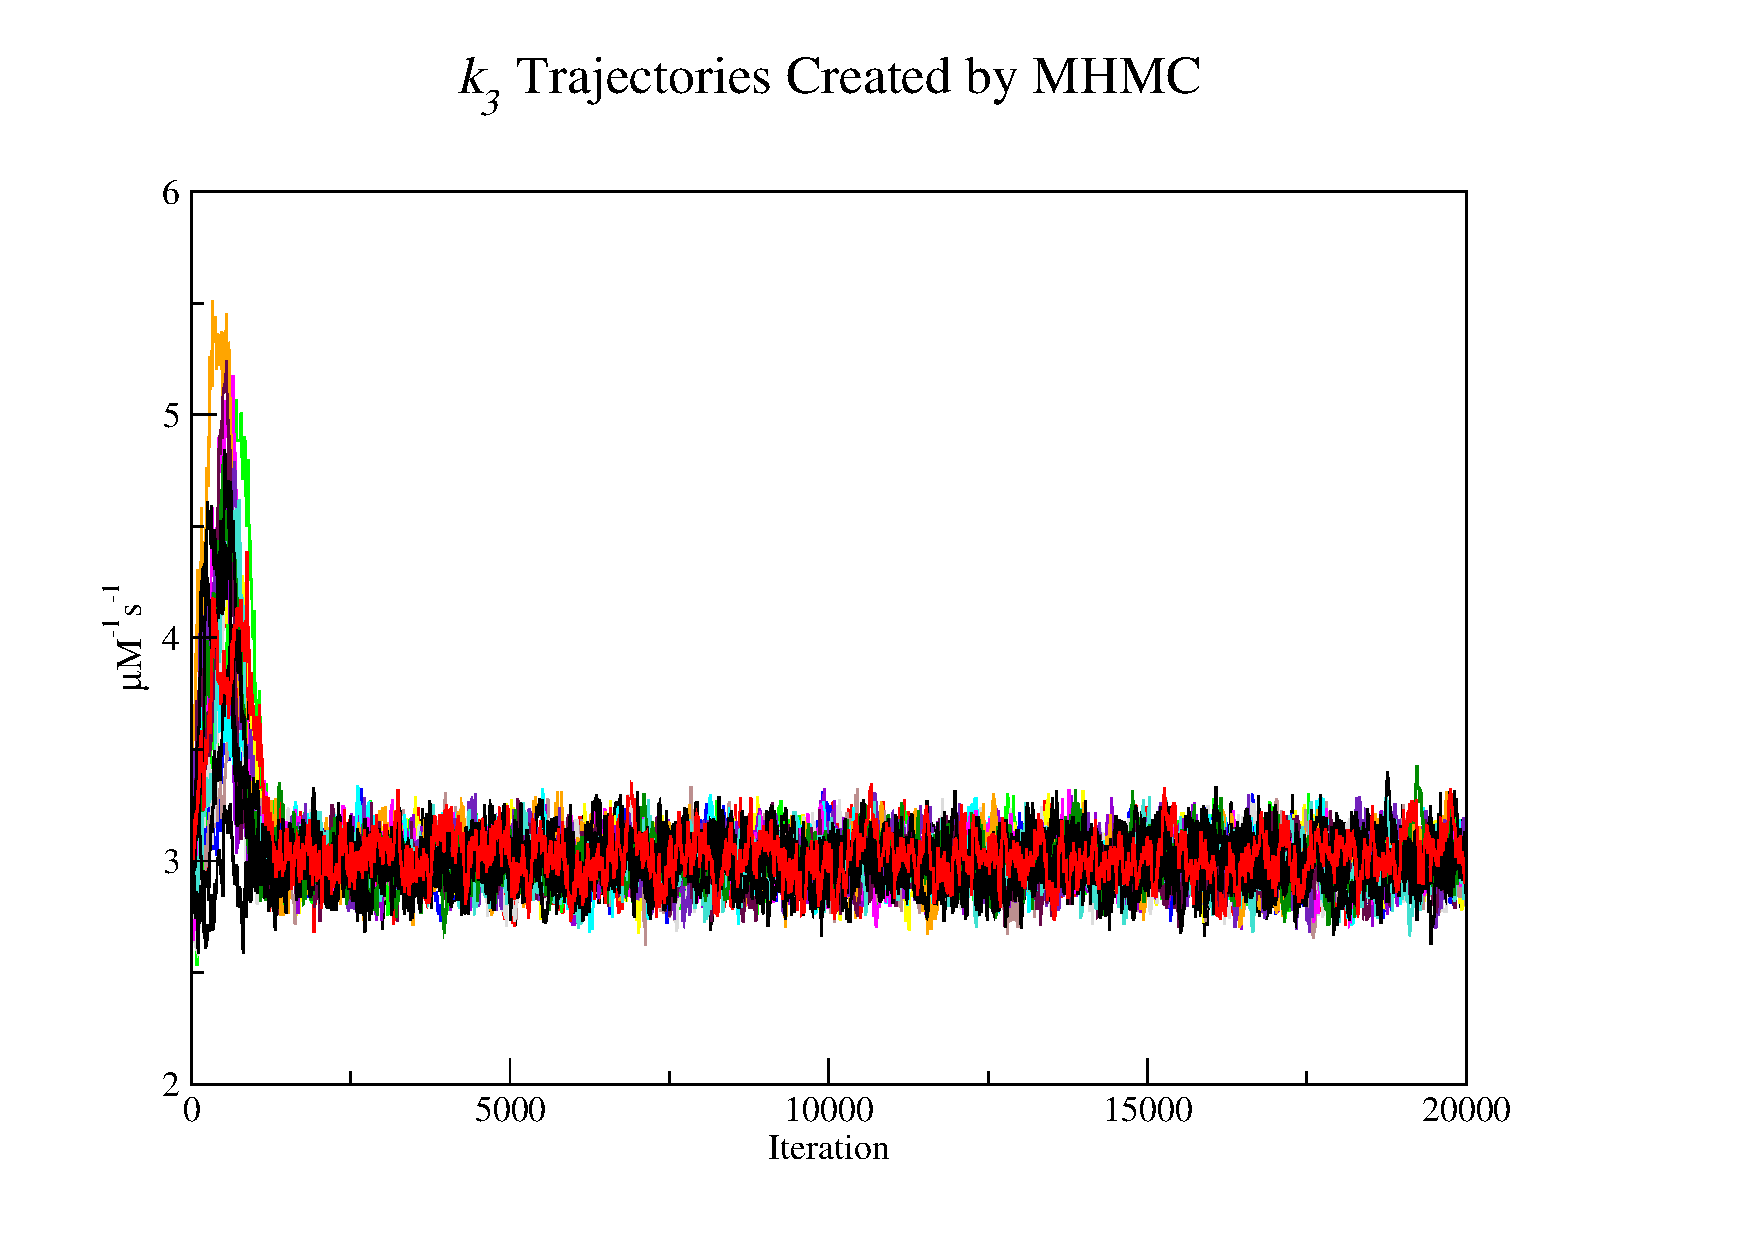
\includegraphics[width=14cm, trim=75px 50px 125px 25px]{./05-oxygenreduction/data/k3s1.pdf}
 % repeatable-oxygen-utilisation-in-mc58.png: 640x480 pixel, 72dpi, 22.58x16.93 cm, bb=0 0 640 480
 \caption[Individual parameter trajectories for multiple runs on the same experimental dataset]{{\bf Individual parameter trajectories for multiple runs on the same experimental dataset.} This figure shows the trajectories for the same parameter, in this case $k_3$ - the rate constant for \cbbthree{} reduction, from 20 individual runs of parameter estimation upon the same input data. The trajectories show clear convergence after the ``burn-in'' period.
 \label{fig:k3s}}
\end{figure}
\afterpage{\clearpage}

Not all parameters in this stage of the model will produce trajectories like the one shown, as if there is a great deal of freedom as to what value a particular parameter can take without drastically decreasing the \textit{BOF} it will be accepted by the parameter estimation algorithm. In this case the trajectories will not converge, and will ultimately produce a wide probability distribution. This is not necessarily indicative of a problem however, as this output still contains information that can be used in the next stage of parameter estimation with new datasets.

The trajectories above are processed to produce probability distributions given as histograms. The ``burn in'' is discarded and the settled data is then binned and counted. For the datasets used, the burn-in period was 1500 iterations (10,000 for dataset 3). These histogram probabilities are then assigned as the posterior distributions and in turn are used directly as prior probability distributions for new datasets. For simplicity's sake when referring to the distribution of individual parameters for purposes of comparison, these histograms are transformed into log-normal distribution such that they can be represented by two numbers, $\bar{x}$ - the mean, and $\sigma^2$ - the variance.

The posterior probability distributions generated from the three experimental datasets, each started with 20 runs are shown in Figure \ref{fig:oxyposteriors}. In the case of parameters which represent concentrations, such as $X$ and $C$, the concentrations of cytochromes and \cbbthree{} respectively, the individual dataset probability distributions are shown, as they cannot be sensibly combined, and it emphasises the fact that the datasets were different.

\begin{figure}[p]
 \centering
 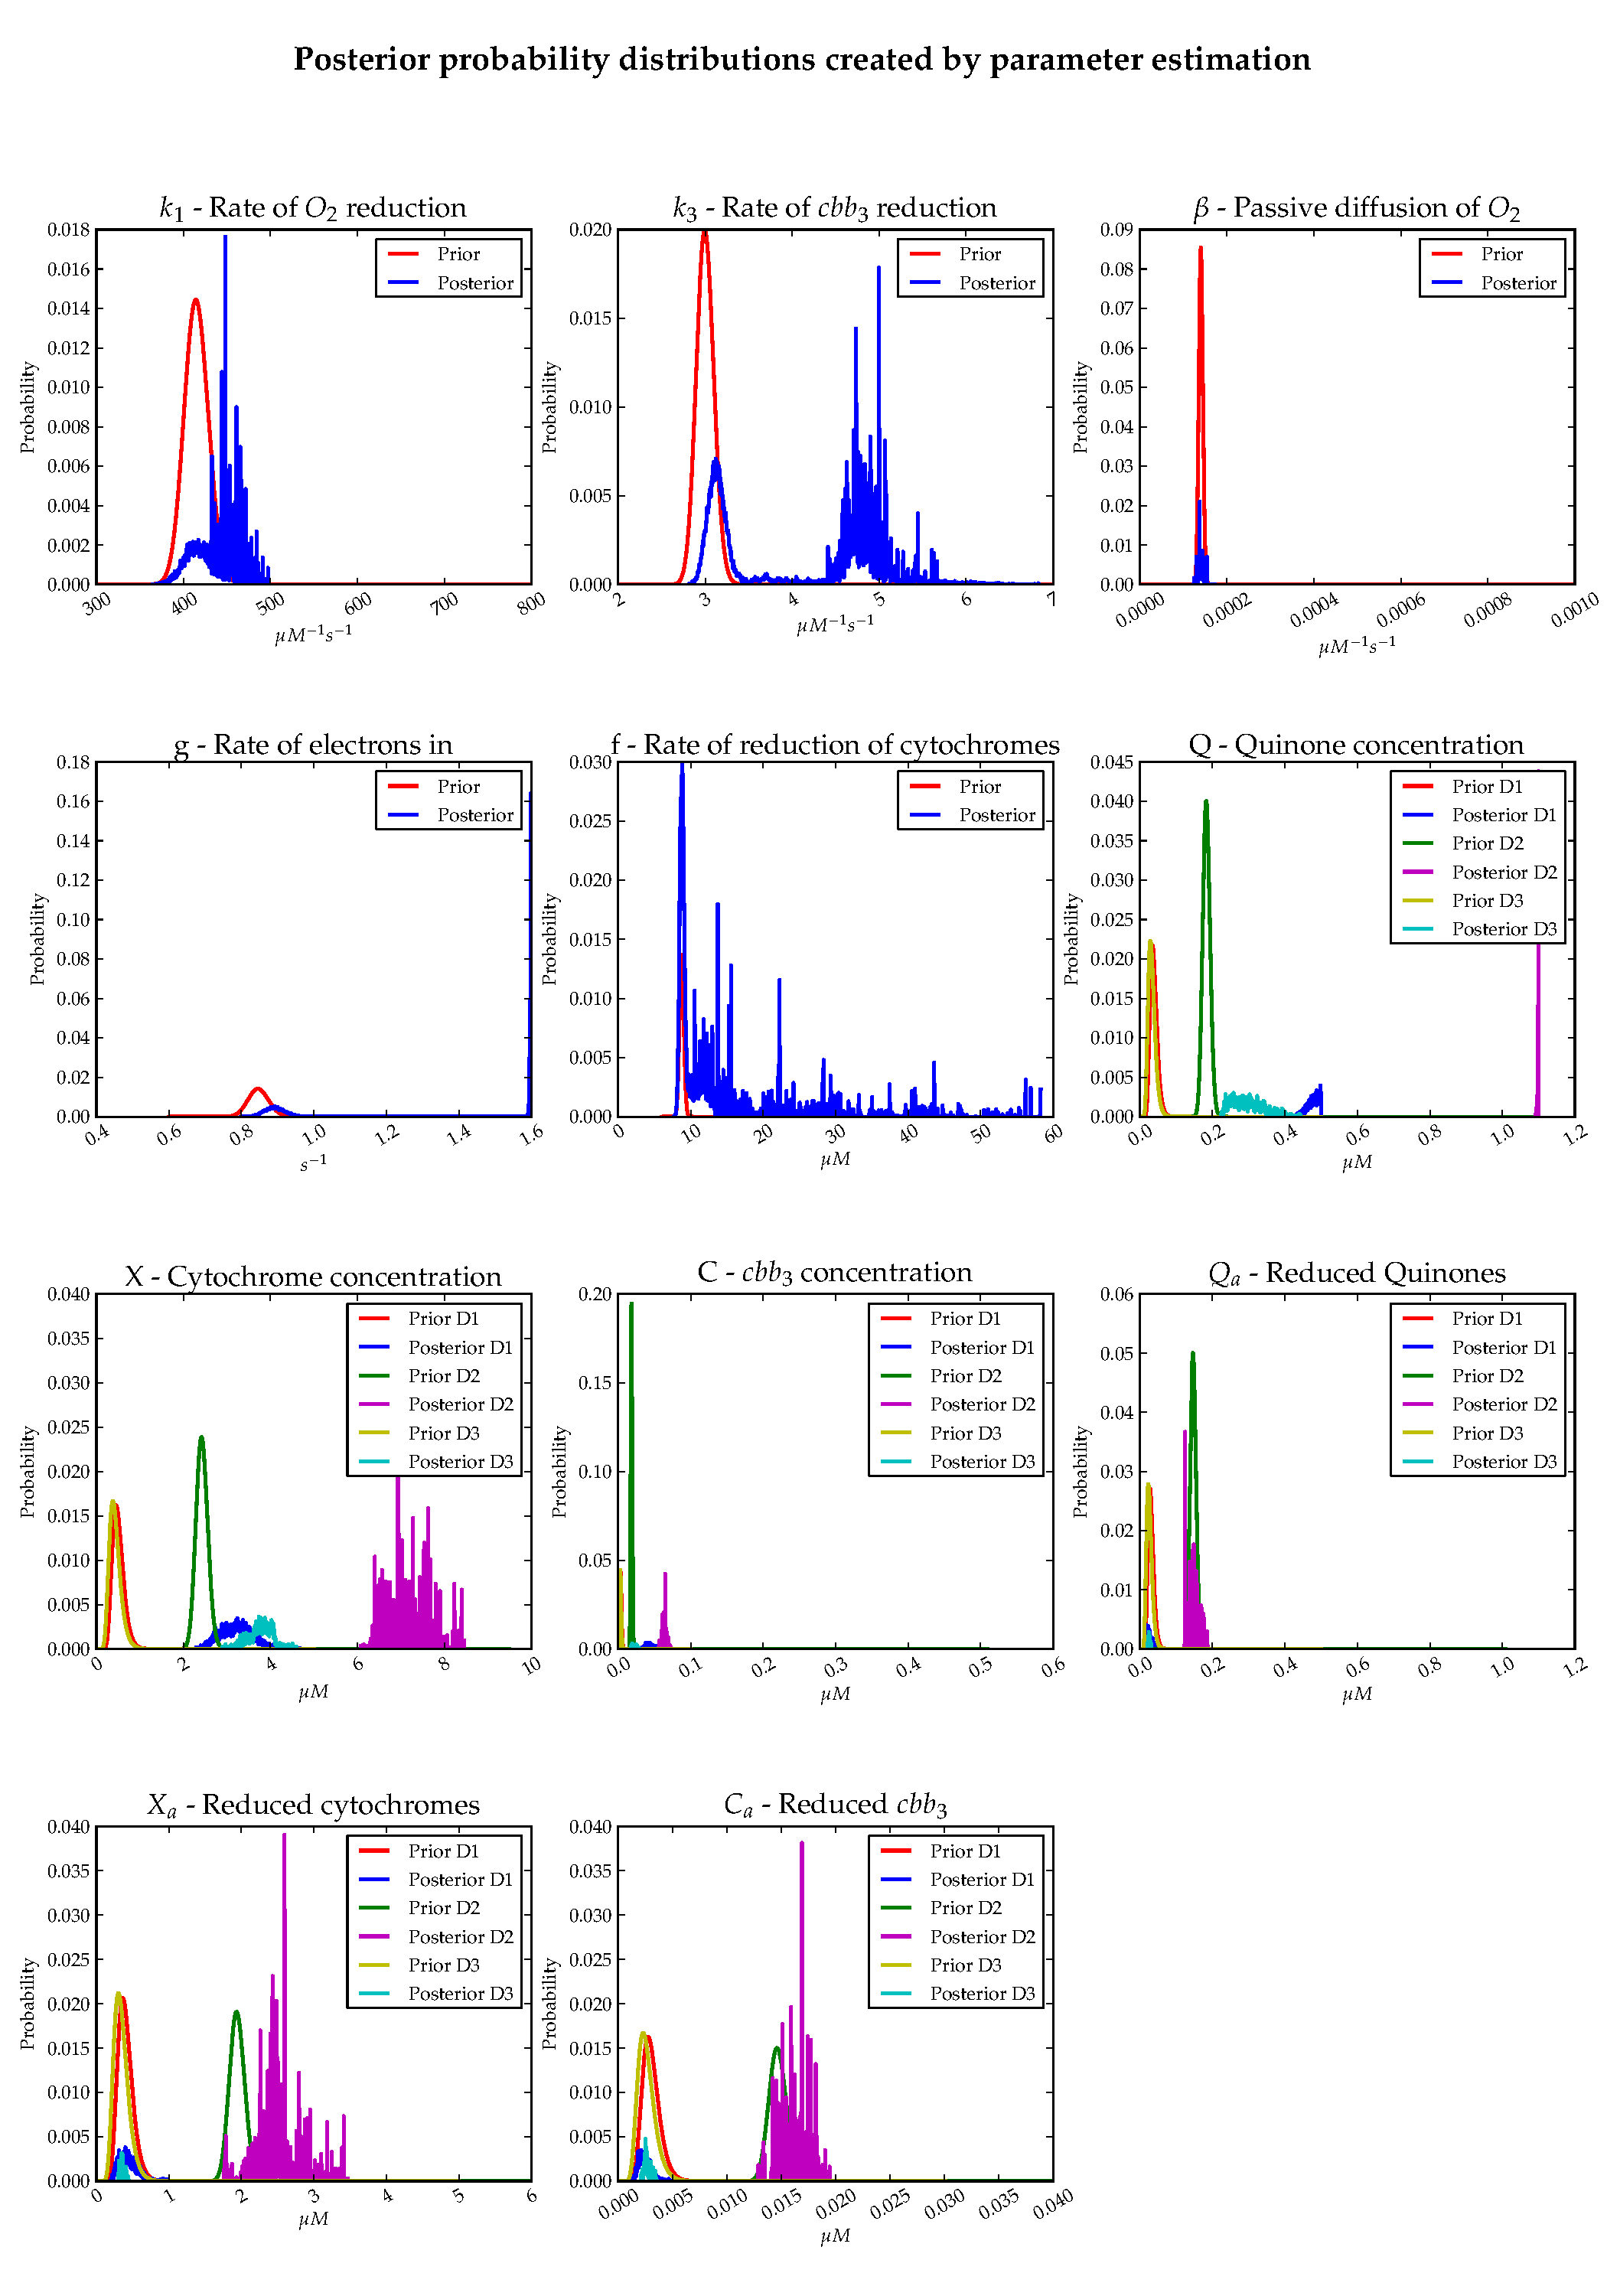
\includegraphics[width=15cm, trim=0cm 0cm 0cm 0cm]{./05-oxygenreduction/data/posteriors1.pdf}
 % posteriors.pdf: 1008x1008 pixel, 72dpi, 35.56x35.56 cm, bb=0 0 1008 1008
 \caption[Posterior probability distributions for oxygen reduction]{{\bf Posterior probability distributions for oxygen reduction}. These are the probability distributions generated by parameter estimation on 3 oxygen reduction datasets. These have been overlaid onto the prior probability distributions used by the parameter estimation algorithm, also shown in Figure \ref{fig:oxypriors}.
 \label{fig:oxyposteriors}}
\end{figure}
\afterpage{\clearpage}

As can be seen from the posterior distributions, the parameter estimation algorithm has not satisfactorily produced posterior distributions that are contained within the bounds of the prior distributions whilst also still managing to fit to the experimental data. This is especially true of the concentration of $Q$, where the Markov-chain has tended towards the upper limit of the input prior distribution. This suggests that the prior distribution for $Q$ is incorrect, with a mean that is possibly as much as $10\times$ too low, and with a variance that is too small, as the parameter estimation algorithm has attempted to increase the value of $Q$ right up to the upper limit of the input distribution. This incorrect value for $Q$ is probably the cause of several of the other distributions being flatter and outside of the main body of their prior distributions. Another interesting observation is that the distribution for $k_3$ shows a distinct bi-modality, however this is quite likely to be an artefact of the parameter estimation algorithm. The left-most region of the bimodal distribution could be caused by the natural bias of the algorithm for values within more likely regions of the prior probability distribution. If this is the case, the right-most region is the ``true'' probability distribution where the increase in likelihood of fitting outweighs the fact that the values selected have a low probability of being selected from the prior distribution. Assuming this is the case, the prior distribution may also be incorrect for $k_3$, but the shape of the posterior distribution may also be directly caused by the more obviously incorrect prior distribution of $Q$.

Since the posterior probability distributions generated at this stage cannot be used as priors for the reasons described above, the prior distributions were altered to try and correct them. These alterations are described in the next section.

%FIXME -> bimodal probability distribution not shown
%Additionally $k_1$, the rate constant for reduction of Oxygen by \cbbthree{} showed bimodality (not shown currently) \textit{and} a very broad range. The bimodal nature of this distribution was not matched in any of the other parameters. This parameter is the last rate constant in the ETC of oxygen reduction, so it is quite possible that the rate limiting steps are in the previous stages of the ETC and thus in the parameter estimation system $k_1$ essentially becomes ``free'', and could be the reason for poor fitting at lower oxygen concentrations.

%Some of the posterior probability distributions appear to have expanded outside their prior bounds. I am fairly certain that this is not an error and that samples \textit{are} being taken from the prior distributions, but rather that the prior distributions were sufficiently incorrect that the penalty for selecting a parameter value from the prior distribution which is very unlikely is outweighed by the large increase in likelihood that this affords.

\subsubsection{Secondary Prior Probability Distributions}
To improve the prior probability distribution to counteract the behaviour seen in the section above, a number of changes were made to the distribution parameters. All of the rate constant and total concentration parameters were flattened out, that is to say the variance was increased. In addition the mean value for $Q$ was increased tenfold since the previously described results showed this value was far too low. The parameters for reduced enzyme concentration were not altered, as the ODE solver is accurate enough to correct these immediately. The values required to create the updated prior probability distributions are shown in Table \ref{tab:oxyProbstat1}.
\begin{table}[h]%needs to be 'here' as section is short
\renewcommand{\arraystretch}{1.5}
\begin{center}
\begin{tabular}{cccc|cccc}
\toprule
\textbf{Parameter} && ${\bar{x}}$ & $\sigma$ & \textbf{Parameter} && ${\bar{x}}$ & $\sigma$\\
\midrule
$k_1$ && 415 & 30.93 & X && 3.97 & 0.424\\
$k_3$ && 3 & 0.316 & C && 0.03 & 0.003\\
$\beta$ && 0.00014 & $4.67\times 10^{-6}$ & $Q_a$ && 0.24 & 0.008\\
g && 0.847 & 0.089 & $X_a$ && 3.176 & 0.105\\
f && 8.749 & 1.732 & $C_a$ && 0.024 & 0.0008\\
Q && 3 & 0.1\\
\bottomrule
\end{tabular}
\end{center}
\caption[Second Prior Probability Table]{{\bf Prior Probability Table} This table shows the prior means and variances used to create lognormal distributions to be used as the prior probability distributions.
\label{tab:oxyProbstat1}}
\end{table}
\afterpage{\clearpage}

A graphical representation of the data in Table \ref{tab:oxyProbstat1}, the initial probability distributions used to start the Monte-Carlo run are shown in Figure \ref{fig:oxypriors1}.
%lbrt
\begin{figure}[p]
 \centering
 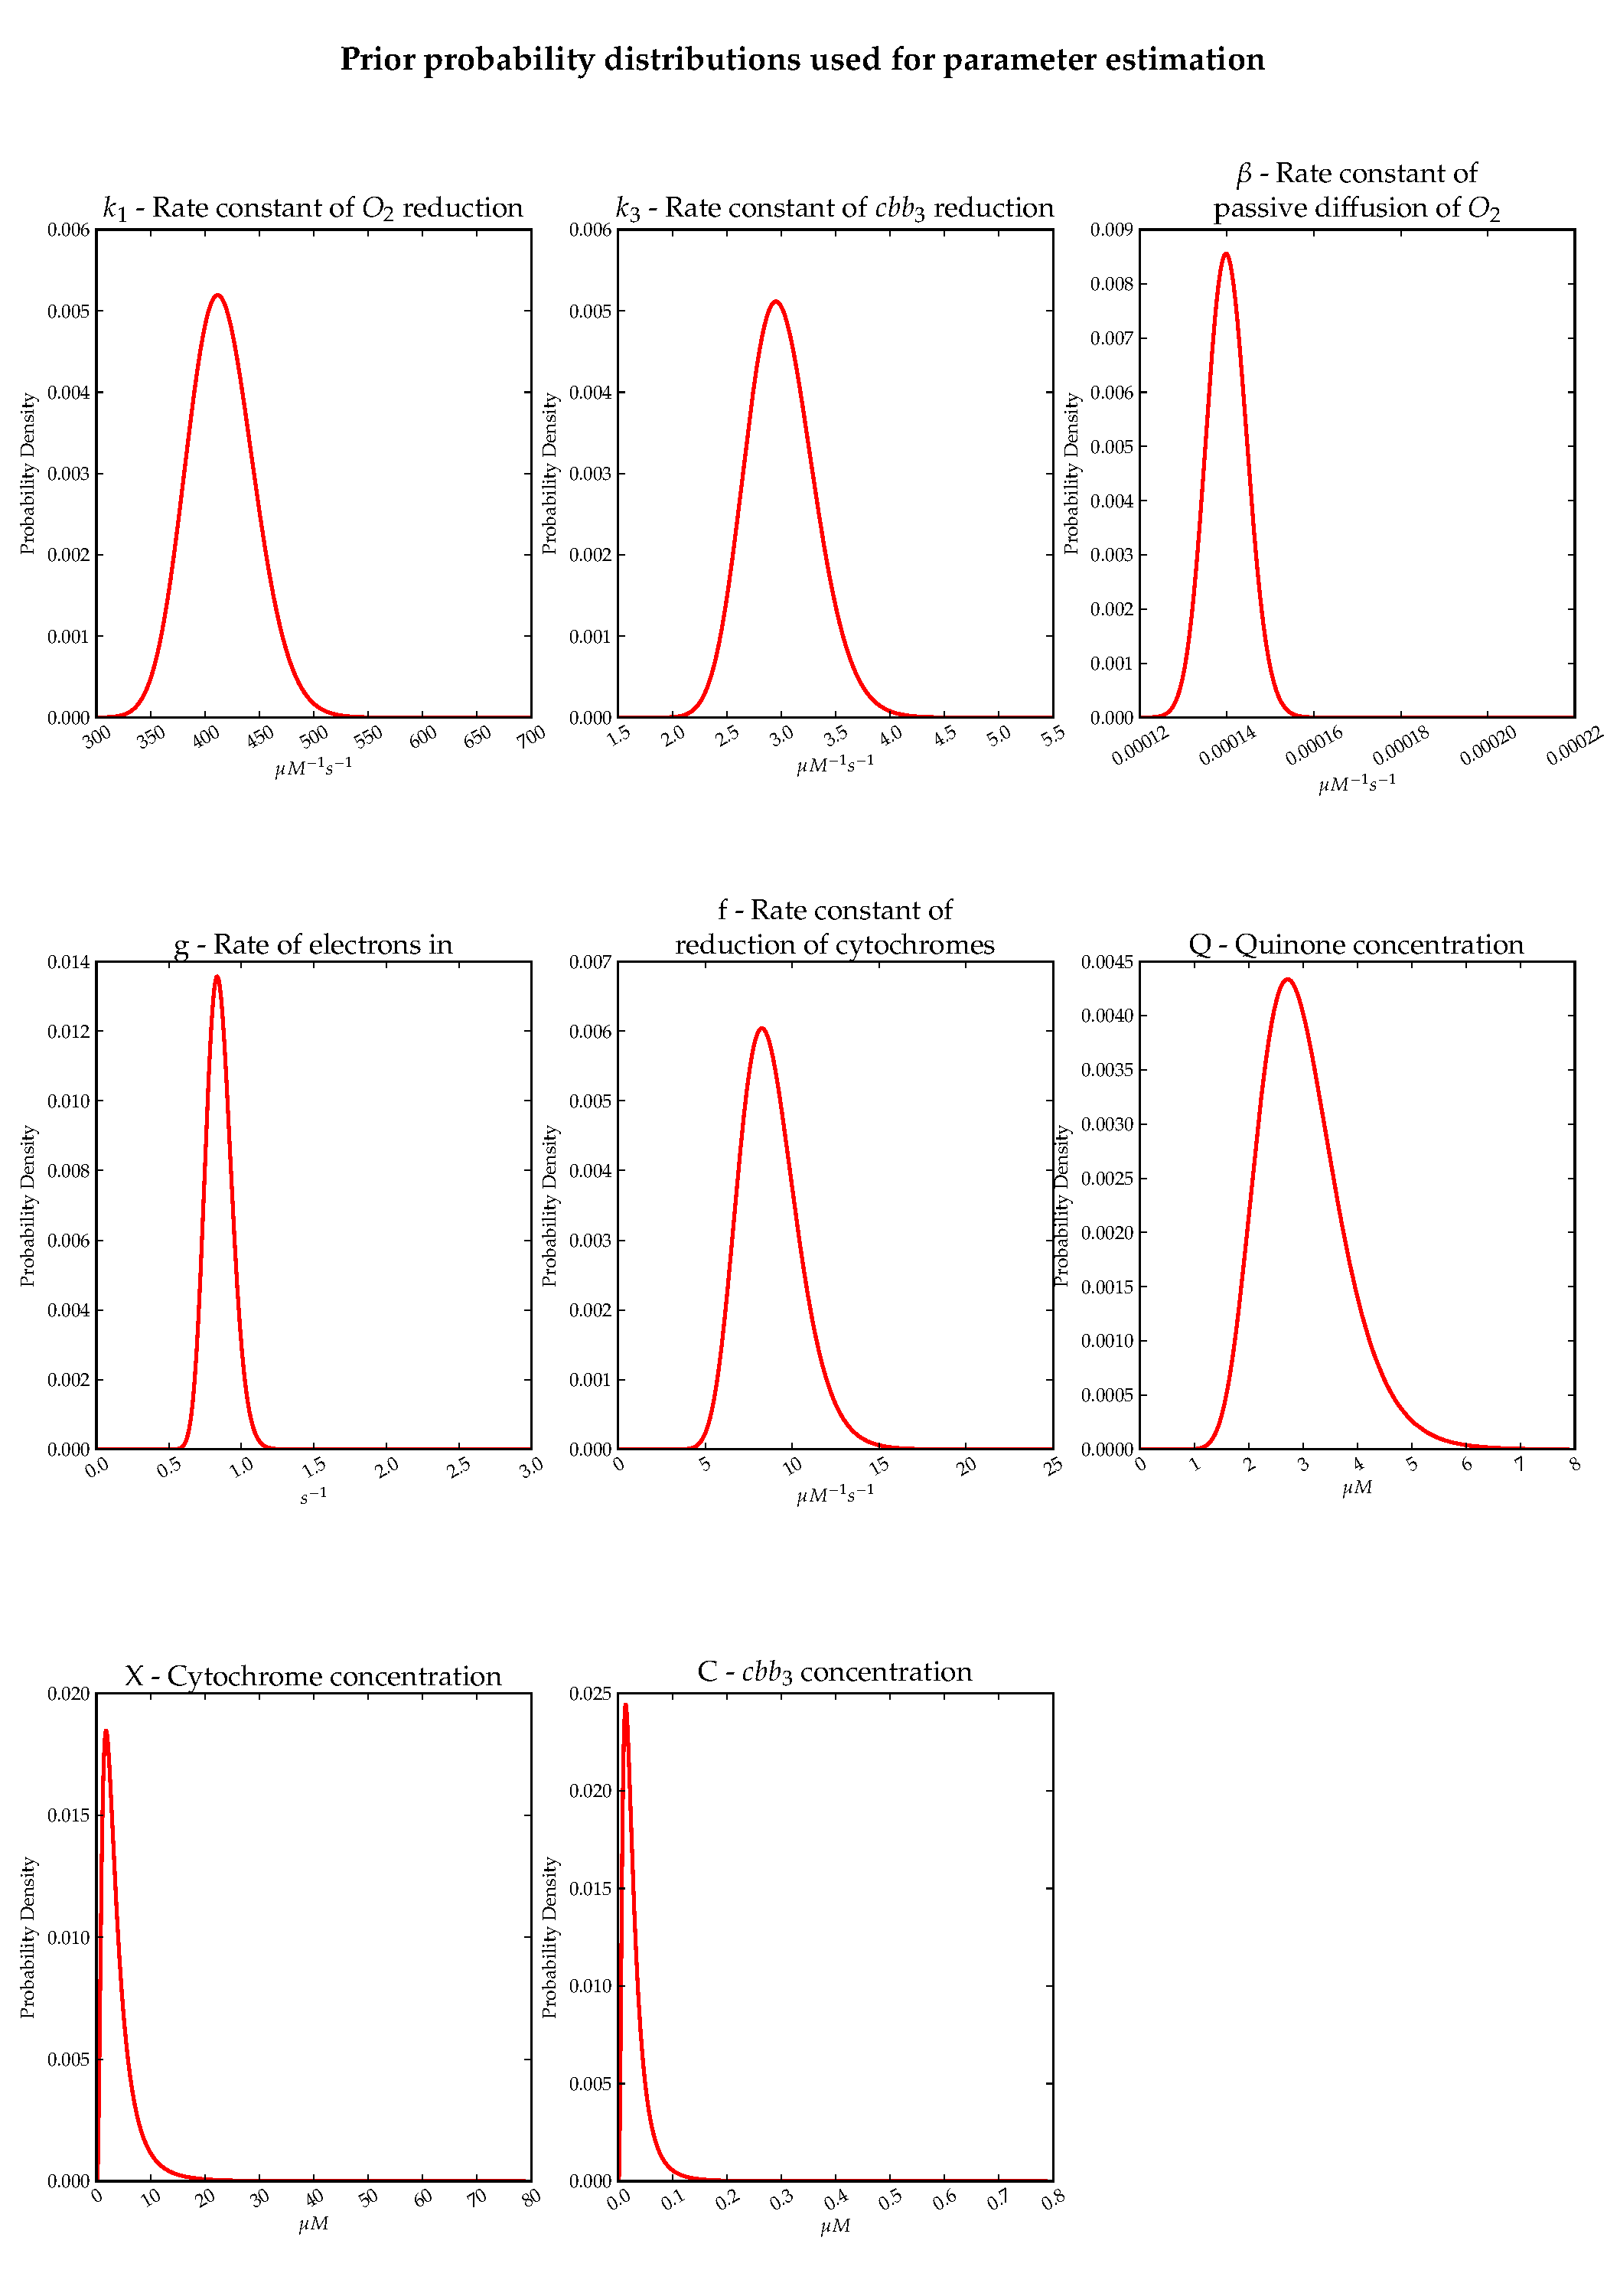
\includegraphics[width=15cm, trim=0cm 0cm 0cm 0cm]{./05-oxygenreduction/data/priors2.pdf}
 % priors.pdf: 1008x1008 pixel, 72dpi, 35.56x35.56 cm, bb=0 0 1008 1008
 \caption[Prior probability distributions for oxygen reduction]{{\bf Prior probability distributions for oxygen reduction}. These are the probability distributions used as priors by the parameter estimation algorithm.
 \label{fig:oxypriors1}}
\end{figure}
%\afterpage{\clearpage}
\subsubsection{Secondary Parameter Estimation Results}
The posterior probability distributions for this second attempt were generated in the same way as described previously for the first attempt.

The second attempt at parameter estimation, revealed an issue with the input datasets that were being used. The first dataset contains no information about what happens to the rate of oxygen reduction once oxygen concentration approaches zero, as the experimental data does not extend this far. The second and third datasets do contain this information as they show complete oxygen reduction to zero, in addition to several seconds of data after that point. This can be seen in Figure \ref{fig:o2data}.

The result of dataset 1 lacking this additional feature is that the parameter estimation algorithm was able to over-sample from the prior distributions as there was no significant difference in goodness-of-fit between ``in prior'' and ``out of prior'' parameter values. If these distributions were to have been included in the overall posterior probability distributions for oxygen reduction they would have skewed the distributions towards the priors rather than their true values. The posterior distributions for dataset 1 are shown in Figure \ref{fig:dataset1posterior}.
%lbrt
\begin{figure}[p]
 \centering
 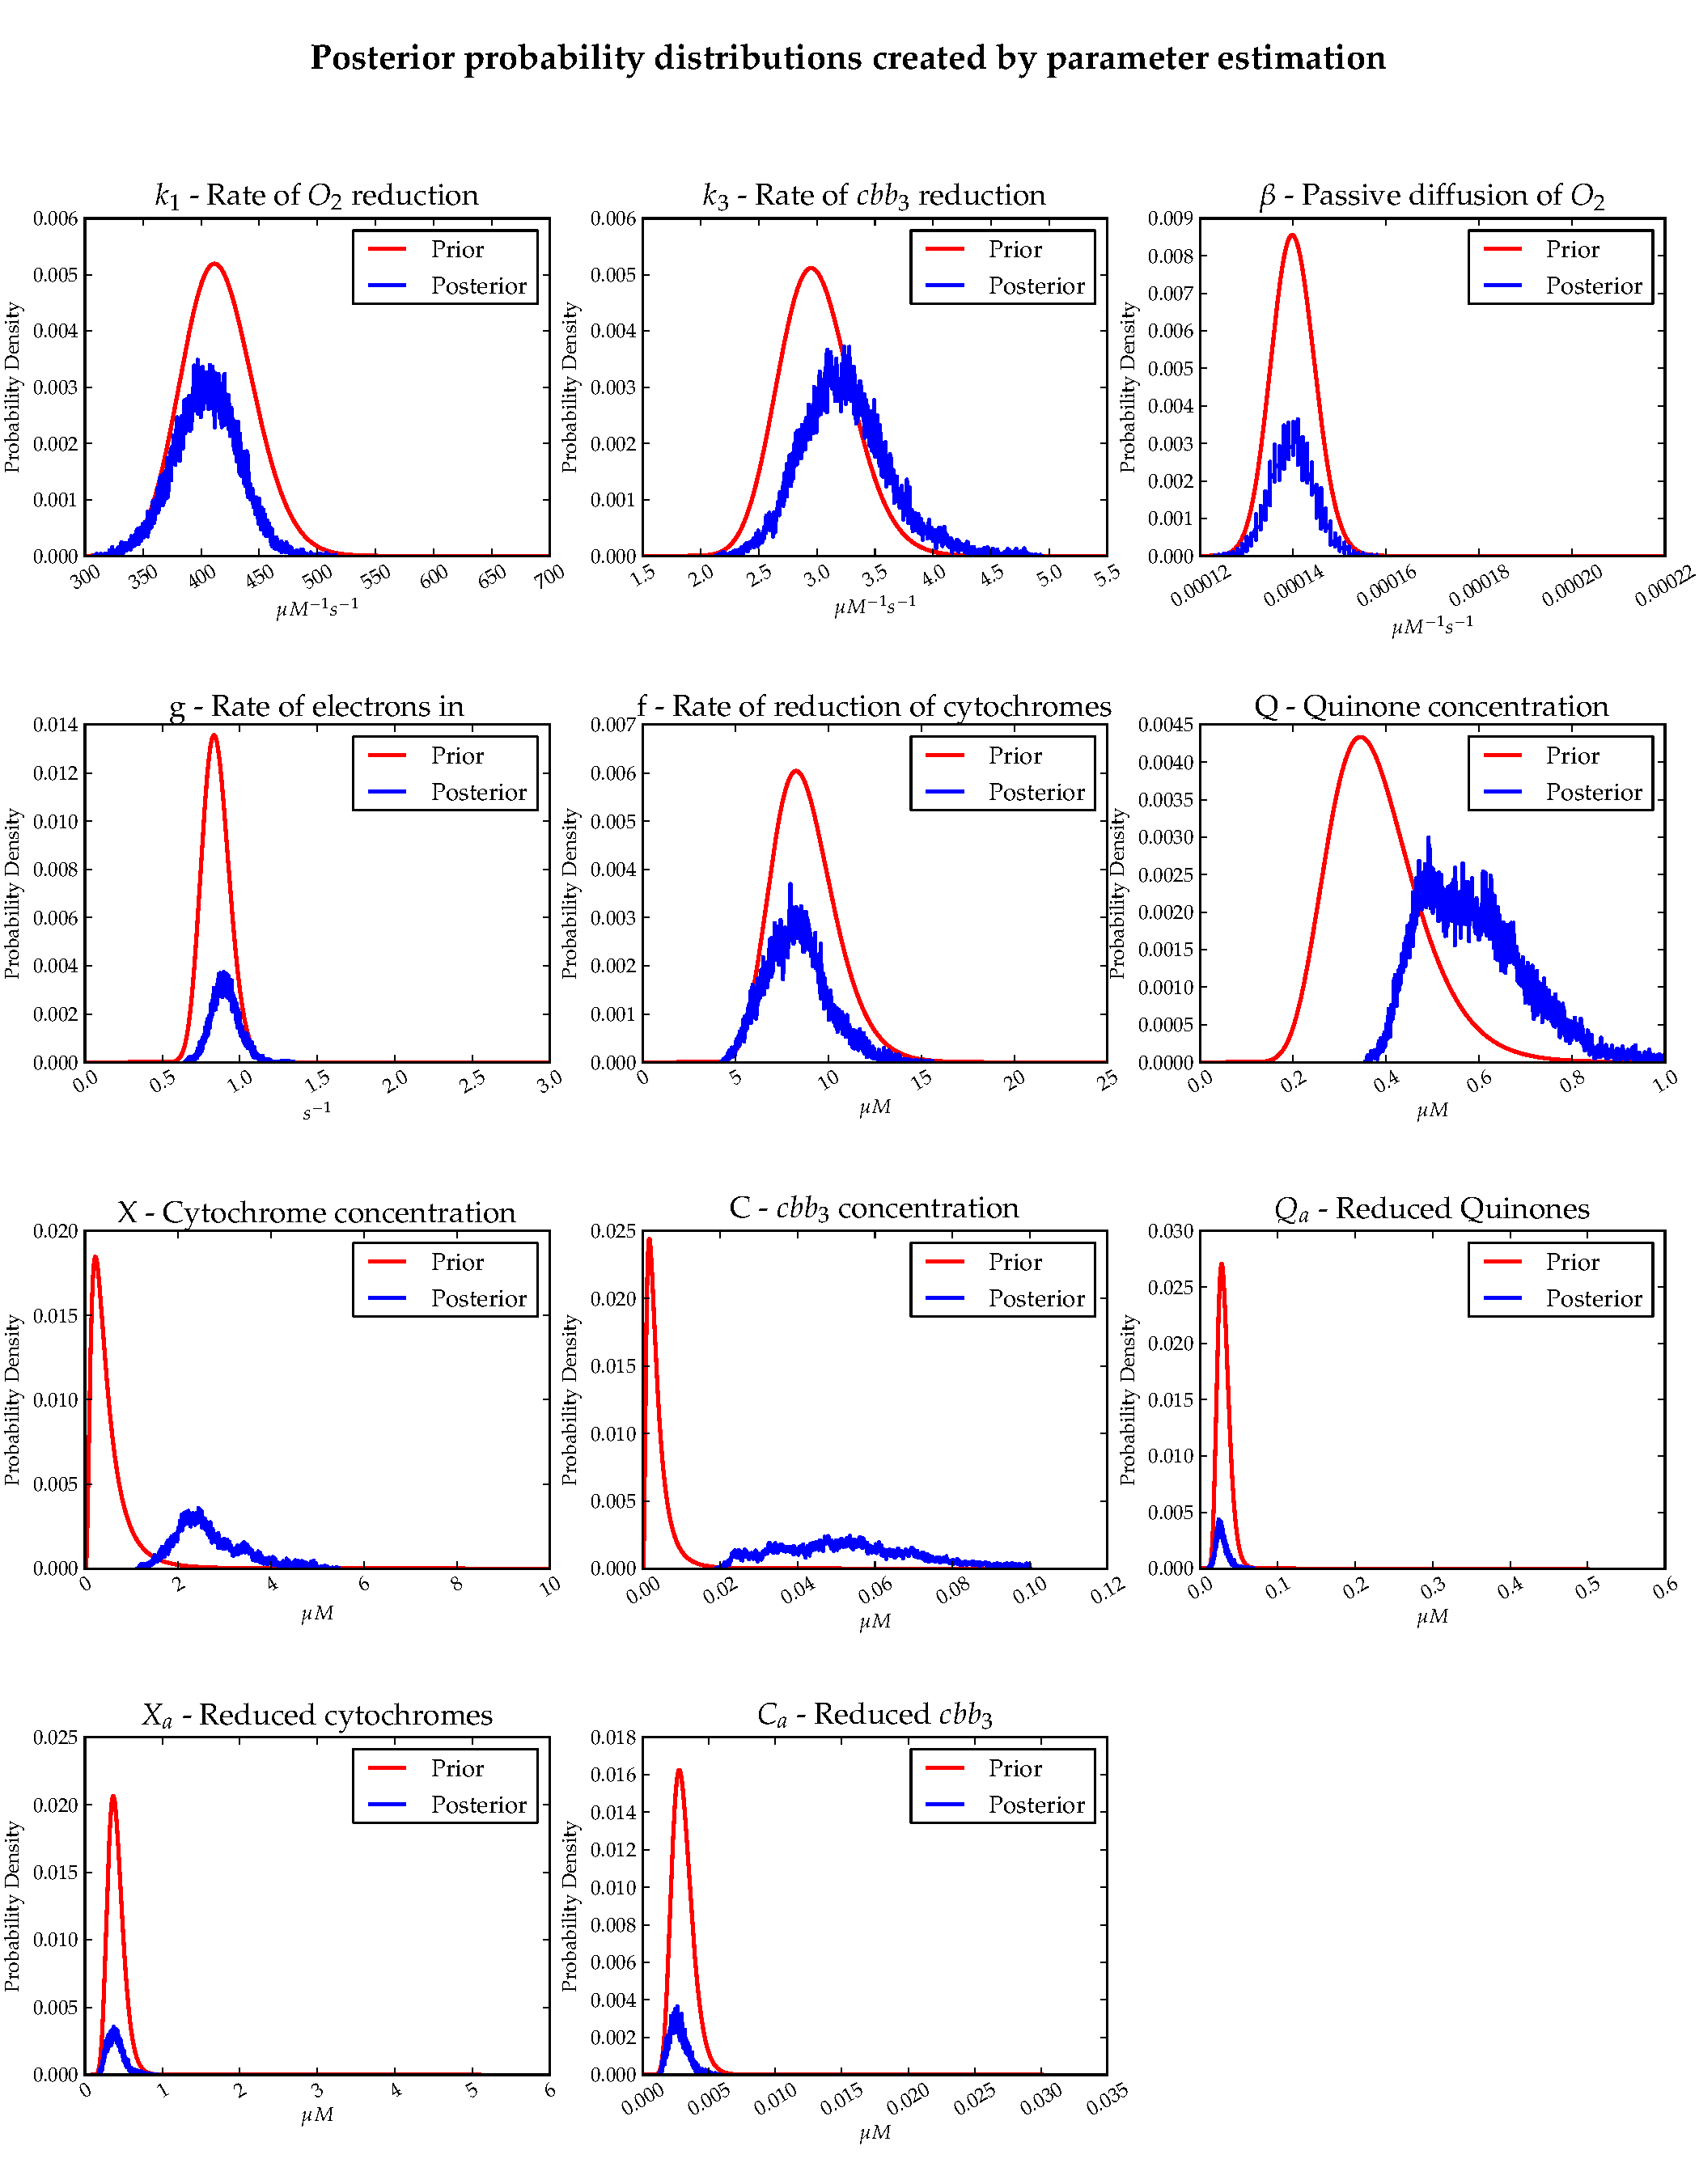
\includegraphics[width=15cm, trim=0cm 0cm 0cm 0cm]{./05-oxygenreduction/data/oversampling_posteriors.pdf}
 % priors.pdf: 1008x1008 pixel, 72dpi, 35.56x35.56 cm, bb=0 0 1008 1008
 \caption[Oversampled Posterior Distributions]{{\bf Oversampled Posterior Distributions}. The posterior probability distributions for dataset 1 of oxygen reduction are oversampled from the prior probability distributions. This is not directly obvious by the probability distributions alone, but in conjunction with the input dataset which lacks features present in datasets 1 and 2. In this case both $k_1$ and $k_3$ are skewed towards the prior probability distributions, and this causes the distribution of $C$ to be very wide as it can take a very broad range of values without affecting the goodness of fit of the solved data to the experimental data.
 \label{fig:dataset1posterior}}
\end{figure}

The usable posterior probability distributions were therefore generated from the experimental datasets 2 \& 3, each started with 20 runs and are shown in Figure \ref{fig:oxyposteriors1}. In the case of parameters which represent concentrations, such as $X$ and $C$, the concentrations of cytochromes and \cbbthree{} respectively, the individual dataset probability distributions are shown, as they cannot be sensibly combined, and it emphasises the fact that the datasets were different.

In the posterior distributions there still appears to be a degree of bimodality in the distribution of the $k_1$, but this distribution is still contained within the prior bounds, and for the purposes of generating a prior probability distribution for the datasets in the next chapter was altered to produce a lognormal distribution that encompasses the entire posterior distribution. The distribution of $k_3$ is perhaps the most interesting as it shows that the estimates used as priors are most likely incorrect as the posterior distribution has shifted significantly to the right, increasing the mean value of the parameter by a factor of $\approx 1.5 \times$. The other rates are largely similar to their prior distributions suggesting that the priors were good estimates for the actual values. The prior distribution for $Q$ had already been altered as described previously and the new value chosen seems to be a great deal better based on the closeness of the posterior distribution to the altered prior distribution. The concentrations of $X$ and $C$ appear to be underestimated in the prior distributions, as the posteriors show a significant shift to the right as with $k_3$. A comparison between the prior probability distributions and the posterior probability distributions can be seen in Table \ref{tab:oxyPstat}. In this table the obtained distributions have been fitted to lognormal distribution which can be described by 2 parameters, which makes comparing the distributions much easier.
\begin{figure}[p]
 \centering
 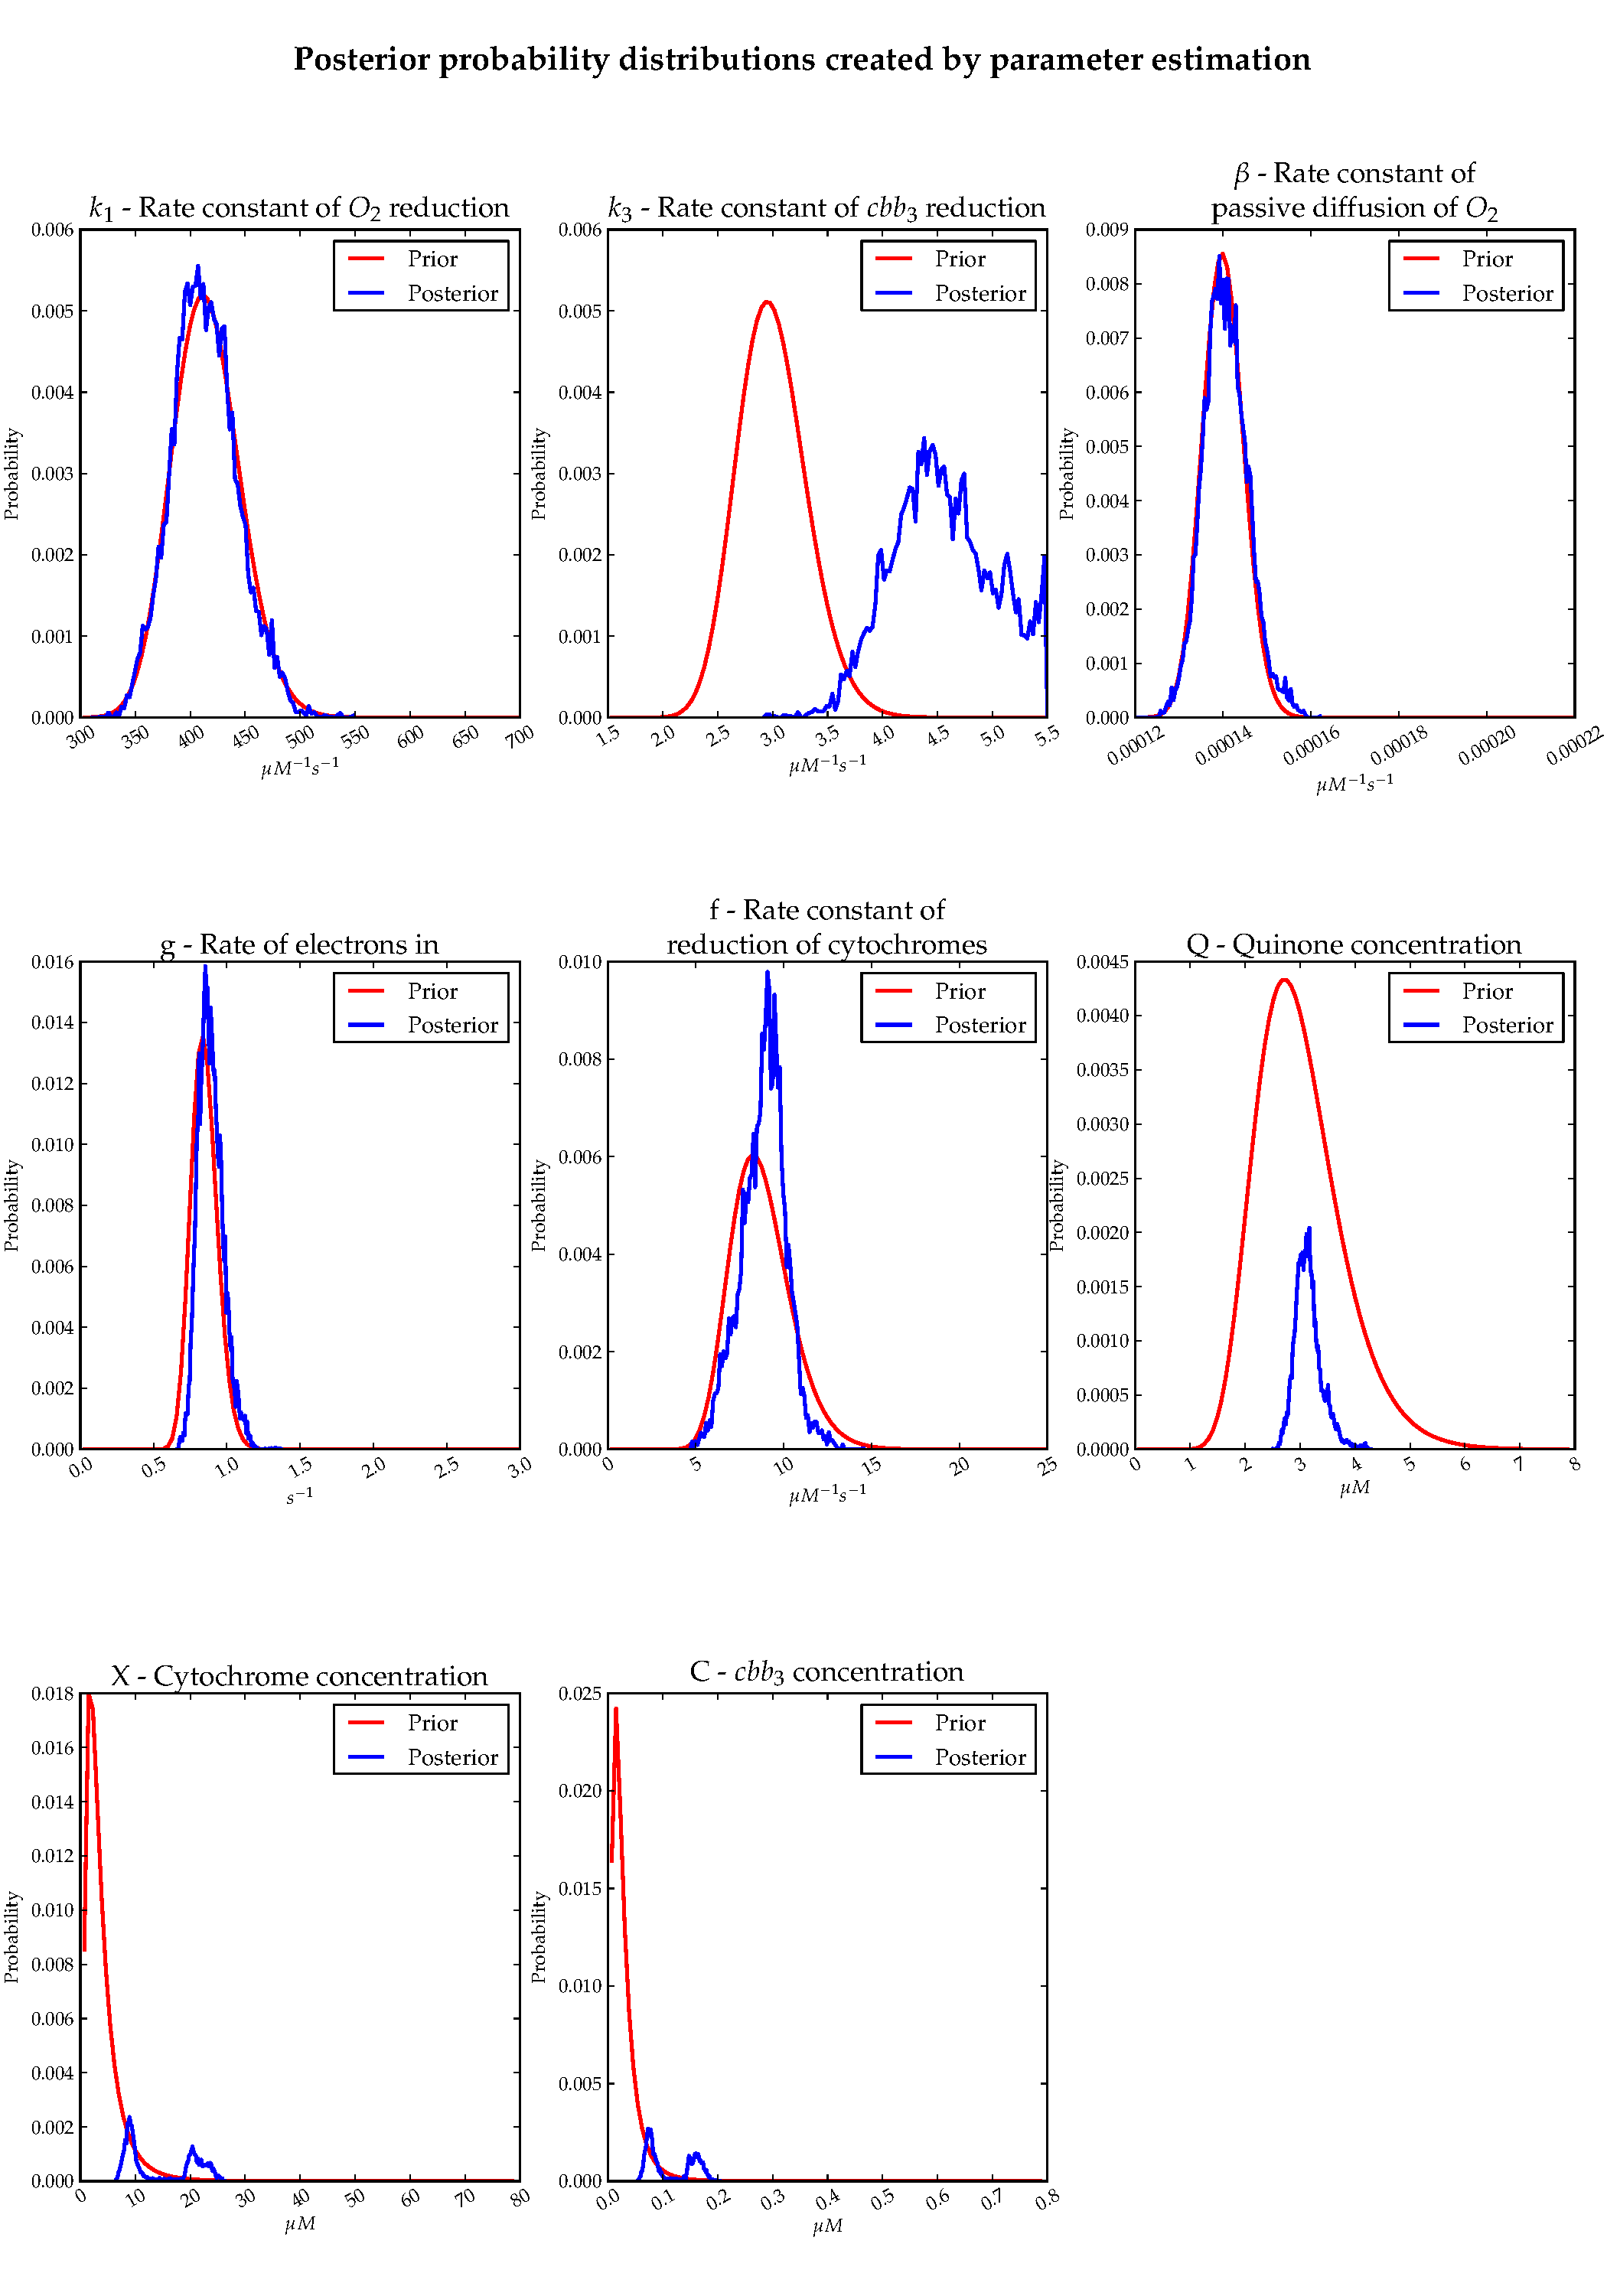
\includegraphics[width=15cm, trim=0cm 0cm 0cm 0cm]{./05-oxygenreduction/data/posteriors3.pdf}
 % posteriors.pdf: 1008x1008 pixel, 72dpi, 35.56x35.56 cm, bb=0 0 1008 1008
 \caption[Posterior probability distributions for oxygen reduction]{{\bf Posterior probability distributions for oxygen reduction}. These are the probability distributions generated by parameter estimation on 2 oxygen reduction datasets. These have been overlaid onto the prior probability distributions used by the parameter estimation algorithm, also shown in Figure \ref{fig:oxypriors1}.
 \label{fig:oxyposteriors1}}
\end{figure}
\afterpage{\clearpage}

\begin{table}[tbp]%needs to be 'here' as section is short
\renewcommand{\arraystretch}{1.5}
\begin{center}
\begin{tabular}{cccccc}
\toprule
& & \multicolumn{2}{c}{\textbf{Priors}} & \multicolumn{2}{c}{\textbf{Posteriors}} \\
\textbf{Parameter} && ${\bar{x}}$ & $\sigma$ & ${\bar{x}}$ & $\sigma$\\
\midrule
$k_1$ && 415 & 30.93 & 413.228 & 30.046\\
$k_3$ && 3 & 0.316 & 4.496 $\uparrow$ & 0.463 $\uparrow$\\
$\beta$ && 0.00014 & $4.67\times 10^{-6}$ & 0.00012 & 0.00017\\
g && 0.847 & 0.089 & 0.889 & 0.089\\
f && 8.749 & 1.732 & 8.707 & 1.35 $\downarrow$\\
Q && 3 & 0.1 & 3.143 & 0.240\\
X && 3.97 & 0.424 & 4.732 $\uparrow$ & 6.707 $\uparrow$\\
C && 0.03 & 0.003 & 0.043 $\uparrow$ & 0.044 $\uparrow$\\
\bottomrule
\end{tabular}
\end{center}
\caption[Posterior Probability Statistics]{{\bf Posterior Probability Statistics.} This table shows the parameters required to create lognormal distributions that describe the prior and posterior probability distributions. The values for the priors are as in Table \ref{tab:oxyProbstat1}. The posterior distributions were generated from datasets 2 \& 3, and where they relate to concentrations, these have been normalised. The lognormal distributions represent best-fits to the actual posterior distributions. Where there are significant differences between the prior and posterior values for either the mean or standard deviation, these are indicated by $\uparrow$ and $\downarrow$.
\label{tab:oxyPstat}}
\end{table}

A graph showing how well the solved output fits the experimental data during the parameter estimation stage is shown in Figure \ref{fig:oxyfinalsolved}. This shows the solved output which achieved the best goodness of fit against the experimental data.
\begin{figure}[tbp]
 \centering
 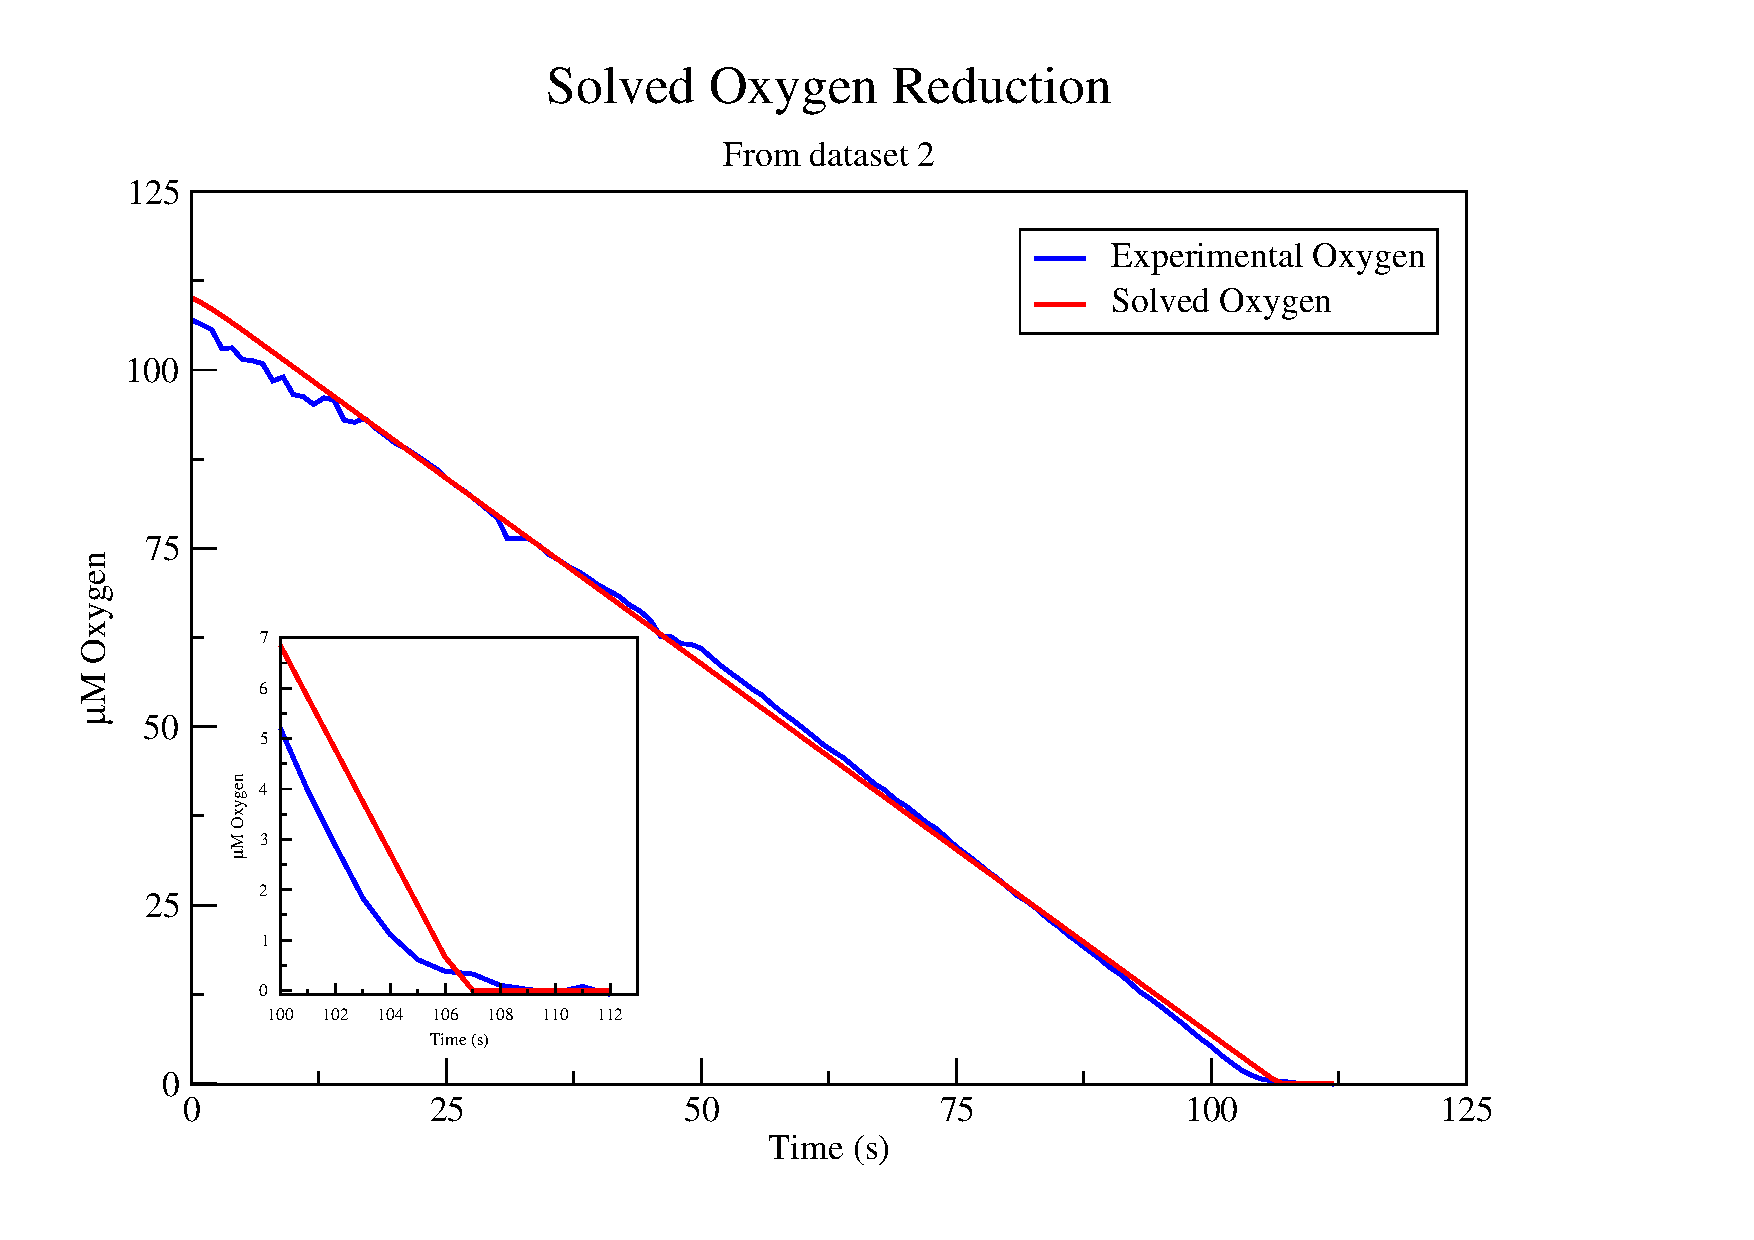
\includegraphics[width=14cm, trim=2cm 1cm 4cm 1cm]{./05-oxygenreduction/data/final_solved.pdf}
 % o2sim.eps: 0x0 pixel, 300dpi, 0.00x0.00 cm, bb=0 0 794 595
 \caption[{Oxygen Reduction in \textit{Neisseria meningitidis}.}]{{\bf Oxygen Reduction in \textit{Neisseria meningitidis}.} This figure shows how well the best solved data fits against the experimental data from dataset 2. The inset shows again, that the solved output is achieving much higher affinity than the experimental data.
 \label{fig:oxyfinalsolved}}
\end{figure}
\afterpage{\clearpage}

\subsubsection{Analysis of Convergence}
It is possible to calculate the degree of convergence of the parameters from the Monte Carlo trajectories using the R statistic introduced by \citet{Gelman1992} and \citet{Brooks1998}. This statistic is a single value that represents how close the trajectories for each individual parameter have come to convergence. The R statistic was calculated using the \textit{Bolstad2}\cite{Curran2011} library for R\cite{RDevelopmentCoreTeam2010}.

Table \ref{tab:oxyRstat} shows the R statistics obtained from the trajectories run for oxygen reduction parameter estimation. The R statistic is a measure of scale-reduction, and fully converged trajectories will have a value of $1.0$ whereas trajectories which have not converged will have values greater than 1 with the magnitude depending on how far away from converging they are. The R statistic shows that all of the rate constants appeared to have converged to a reasonably high degree which could also be seen from the distribution plots. The concentration parameters had converged to a much lesser degree however this was not completely unexpected, as there were a larger number of parameters in the model than were required to fit the experimental data and thus the potential range of parameter values was broad at this stage. The apparent lack of convergence of some parameters at this point was not a problem as with subsequent, more complex datasets, the range of potential parameter values should decrease, allowing the trajectories to converge more easily.
\begin{table}[tbp]%needs to be 'here' as section is short
\renewcommand{\arraystretch}{1.5}
\begin{center}
\begin{tabular}{ccc|ccc}
\toprule
\textbf{Parameter} && \textbf{R value} & \textbf{Parameter} && \textbf{R value}\\
\midrule
$k_1$ && 1.38 & f && 1.65\\
$k_3$ && 1.36 & Q && 2.37\\
$\beta$ && 1.09 & X && 11.93\\
g && 1.57 & C && 9.44\\
\bottomrule
\end{tabular}
\end{center}
\caption[Gelman-Rubin Convergence Statistic]{{\bf Gelman-Rubin Convergence Statistic.} This table shows the Gelman-Rubin Convergence statistic for all the Markov chains from datasets 2 \& 3. For parameters which are concentrations, the statistic relates to the values after normalisation (data is normalised based on initial oxygen reduction rate). Concentration parameters exhibit greater inter-dataset differences even after normalisation thus giving high R statistic values. The intra-dataset values are lower.
\label{tab:oxyRstat}}
\end{table}

\subsubsection{Analysis of Correlation}
Given the large number of parameters, and the simple form of the experimental data it is quite likely that a number of the parameters will be correlated with one another. This effect should also have been exacerbated at this stage due to the limited constraints (by virtue of wide prior probabilities) on the ranges of values that parameters can take. In order to investigate this a set of correlation matrices were constructed by calculating the Pearson's Product-Moment Correlation Coefficient for each of the parameters. This value provides the direction of correlation as indicated by the sign, and the degree of linearity as indicated by the magnitude. A positive correlation indicates that as the value of one parameter increases, the other increases also. A negative correlation indicates that as the value of one parameter increases, the other decreases.

The upper-triangle correlation matrices are shown in Figures \ref{tab:oxyregress1} \& \ref{tab:oxyregress2} and were constructed by concatenating all the trajectories created by the parameter estimation system (discarding the burn-in) together and the Pearson's Product-Moment Correlation Coefficient calculated for each combination for each dataset. The datasets were analysed separately to allow examination of intra dataset correlation. The matrices are upper-triangle only as the lower triangle is a duplicate of the same data. The diagonals are shown in grey as they are not useful data since the correlation of X against X is always 1.
%\begin{landscape}
\begin{table}[p]
\setlength{\tabcolsep}{5pt}
\renewcommand{\arraystretch}{1.5}
  \centering
  \rotatebox{90}{
  \begin{minipage}{24.4cm}
  \centering
  \begin{tabular}{|c|c|c|c|c|c|c|c|c|c|}
    \hline
    \cellcolor{dark-gray} & \cellcolor{dark-gray}$k_1$ & \cellcolor{dark-gray}$k_3$ & \cellcolor{dark-gray}$\beta$ & \cellcolor{dark-gray}g & \cellcolor{dark-gray}f & \cellcolor{dark-gray}Q & \cellcolor{dark-gray}X & \cellcolor{dark-gray}C \\
    \hline
    \cellcolor{dark-gray}$k_1$ & \cellcolor{light-gray}$1$ & 0.010353 & 0.007923 & 0.033363 & -0.009149 & -0.004965 & 0.017719 & -0.029593 \\
    \hline
    \cellcolor{dark-gray}$k_3$ & \cellcolor{light-gray} & \cellcolor{light-gray}$1$ & -0.015159 & -0.110244 & 0.050016 & -0.020452 & \cellcolor{orange}-0.318503 & \cellcolor{orange}-0.479758 \\
    \hline
    \cellcolor{dark-gray}$\beta$ & \cellcolor{light-gray} & \cellcolor{light-gray} & \cellcolor{light-gray}$1$ & 0.002275 & -0.009439 & -0.003051 & 0.017707
 & -0.003679 \\
    \hline
    \cellcolor{dark-gray}g & \cellcolor{light-gray} & \cellcolor{light-gray} & \cellcolor{light-gray} & \cellcolor{light-gray}$1$ & -0.042492 & -0.123088 & 0.122328 & -0.093617 \\
    \hline
    \cellcolor{dark-gray}f & \cellcolor{light-gray} & \cellcolor{light-gray} & \cellcolor{light-gray} & \cellcolor{light-gray} & \cellcolor{light-gray}$1$ & -0.052359 & -0.060664 & -0.029025 \\
    \hline
    \cellcolor{dark-gray}Q & \cellcolor{light-gray} & \cellcolor{light-gray} & \cellcolor{light-gray} & \cellcolor{light-gray} & \cellcolor{light-gray} & \cellcolor{light-gray}$1$ & 0.061756 & -0.086643 \\
    \hline
    \cellcolor{dark-gray}X & \cellcolor{light-gray} & \cellcolor{light-gray} & \cellcolor{light-gray} & \cellcolor{light-gray} & \cellcolor{light-gray} & \cellcolor{light-gray} & \cellcolor{light-gray}$1$ & \cellcolor{orange}-0.658657 \\
    \hline
    \cellcolor{dark-gray}C & \cellcolor{light-gray} & \cellcolor{light-gray} & \cellcolor{light-gray} & \cellcolor{light-gray} & \cellcolor{light-gray} & \cellcolor{light-gray} & \cellcolor{light-gray} & \cellcolor{light-gray}$1$ \\
    \hline
  \end{tabular}
  \caption[Regression Analysis of Oxygen Reduction Parameters]{{\bf Regression Analysis of Oxygen Reduction Parameters for Dataset 2.} This table shows the $R$ values from linear regression analysis on the combined parameter trajectories for Oxygen reduction. Parameters with high correlation have been coloured green ($R>0.8$) and those with moderation correlation have been coloured orange ($0.8>R>0.3$).
  \label{tab:oxyregress1}}
  \end{minipage}
  }
\end{table}
\afterpage{\clearpage}
%\end{landscape}
\begin{table}[p]
\setlength{\tabcolsep}{5pt}
\renewcommand{\arraystretch}{1.5}
  \centering
  \rotatebox{90}{
  \begin{minipage}{24.4cm}
  \centering
  \begin{tabular}{|c|c|c|c|c|c|c|c|c|c|}
    \hline
    \cellcolor{dark-gray} & \cellcolor{dark-gray}$k_1$ & \cellcolor{dark-gray}$k_3$ & \cellcolor{dark-gray}$\beta$ & \cellcolor{dark-gray}g & \cellcolor{dark-gray}f & \cellcolor{dark-gray}Q & \cellcolor{dark-gray}X & \cellcolor{dark-gray}C \\
    \hline
    \cellcolor{dark-gray}$k_1$ & \cellcolor{light-gray}$1$ & -0.002964 & 0.149765 & 0.083521 & 0.13787 & -0.088977 & -0.006116 & 0.011541 \\
    \hline
    \cellcolor{dark-gray}$k_3$ & \cellcolor{light-gray} & \cellcolor{light-gray}$1$ & 0.032078 & -0.046175 & 0.05076 & -0.102051 & \cellcolor{orange}-0.634699 & \cellcolor{orange}-0.4545 \\
    \hline
    \cellcolor{dark-gray}$\beta$ & \cellcolor{light-gray} & \cellcolor{light-gray} & \cellcolor{light-gray}$1$ & 0.050182 & -0.007235 & -0.120098 & 0.103706 & -0.135299 \\
    \hline
    \cellcolor{dark-gray}g & \cellcolor{light-gray} & \cellcolor{light-gray} & \cellcolor{light-gray} & \cellcolor{light-gray}$1$ & 0.104896 & \cellcolor{orange} -0.473135 & -0.150992 & 0.199826 \\
    \hline
    \cellcolor{dark-gray}f & \cellcolor{light-gray} & \cellcolor{light-gray} & \cellcolor{light-gray} & \cellcolor{light-gray} & \cellcolor{light-gray}$1$ & -0.127323 & -0.090914 & -0.022676 \\
    \hline
    \cellcolor{dark-gray}Q & \cellcolor{light-gray} & \cellcolor{light-gray} & \cellcolor{light-gray} & \cellcolor{light-gray} & \cellcolor{light-gray} & \cellcolor{light-gray}$1$ & 0.09321 & -0.116721 \\
    \hline
    \cellcolor{dark-gray}X & \cellcolor{light-gray} & \cellcolor{light-gray} & \cellcolor{light-gray} & \cellcolor{light-gray} & \cellcolor{light-gray} & \cellcolor{light-gray} & \cellcolor{light-gray}$1$ & \cellcolor{orange}-0.379235 \\
    \hline
    \cellcolor{dark-gray}C & \cellcolor{light-gray} & \cellcolor{light-gray} & \cellcolor{light-gray} & \cellcolor{light-gray} & \cellcolor{light-gray} & \cellcolor{light-gray} & \cellcolor{light-gray} & \cellcolor{light-gray}$1$ \\
    \hline
  \end{tabular}
  \caption[Regression Analysis of Oxygen Reduction Parameters]{{\bf Regression Analysis of Oxygen Reduction Parameters for Dataset 3.} This table shows the $R$ values from linear regression analysis on the combined parameter trajectories for Oxygen reduction. Parameters with high correlation have been coloured green ($R>0.8$) and those with moderation correlation have been coloured orange ($0.8>R>0.3$).
  \label{tab:oxyregress2}}
  \end{minipage}
  }
\end{table}
\afterpage{\clearpage}

The correlation matrices show that most of the model parameters are not correlated with each other, giving low to very low $R$ values. Between the two datasets the only parameters that appear to be correlated are $C$ and $X$ and $k_3$ and $X$, and these are both negative correlations. The negative correlation between $k_3$ and $X$ can be explained by the fact that as the concentration of $X$ decreases, an increase in $k_3$ is required to maintain the same rate of electron flow out of the cytochrome pool. The correlation between $C$ and $X$ can be explained by factoring in the fact that the rate of oxidation of $C$ is very high. This should lead to any reduced \cbbthree{} being oxidised almost straight away. Therefore if the concentration of $X$ increased, it would lead to an increase in the reduction state of $C$ (as there will be more electrons to move from $X$ to $C$), so to maintain the same eventual rate of oxygen reduction (by oxidation of $C$), the concentration of $C$ must decrease. The converse is also true.
The fact that there are intra-dataset correlations that don't appear in both datasets suggests that the rates and concentrations in the two datasets haven't been completely decoupled from the optical density (or in this case the reduction rate proxy for OD). The positions in the electron transport chain of these correlations are shown below, marked by superscript $^\blacktriangle$ and $^\square$.
\begin{equation*}
\xrightarrow{g}Q\xrightarrow{f}X^{\blacktriangle}\xrightarrow{k_3^{\square}}C^{\square\blacktriangle}\xrightarrow{k_1}O_2
\end{equation*}

\subsection{Discussion}
The experimental datasets showed that oxygen reduction in \Nm{} is a simple almost completely linear system with the reductase having a high affinity for oxygen demonstrated by the almost complete lack of non-linearity as oxygen concentration approaches zero. This simple linearity could be very easily have been modelled to a high degree of accuracy with just 2 parameters in a simple $y=-mx+c$ system. Admittedly this would not include the behaviour when the oxygen concentration reaches zero, where the is some non-linearity. However this essentially meant that there were a much larger number of parameters available to fit than were necessary, which lead to over-fitting of the data. The size of the parameter set meant that there were a very large set of potential combinations that would have lead to a similar result, however this was mitigated somewhat by the prior probability distributions given to the algorithm. Even so, this meant that the posterior distributions generated were very wide and therefore allowed much greater freedom for the next dataset to explore the parameter space.

With the knowledge of the underlying transport chain and the affinity of \cbbthree{} for oxygen, a linear reduction of oxygen with high affinity over nearly two orders of magnitude was expected. This was evidenced in the experimental data. It is however remarkable that this behaviour can be modelled with so few components in the model, as it requires significant changes in the reduction states of the enzymes to achieve this.

Perhaps the most interesting new piece of data to come out of this first round of parameter estimation is the discovery that the literature value used for the concentration of quinones - Q - in the cell was at lest an order of magnitude too low. This can be explained however by the fact that the literature value used is not for the same bacteria, and there were a number of assumptions made about \Nsm{} cell size and weight.
%TODO reduction state plots